\chapter{Phân lớp chữ số MNIST Handwritten bằng ANN}

\section{Tổng quan}

Từ phần EDA của Lab 02, có ba insight chính được giữ lại cho Lab 03. Thứ nhất, MNIST là bộ dữ liệu khá sạch, kích thước ảnh đồng nhất và độ tương phản giữa nét chữ với nền đủ rõ để một ANN thuần vẫn có thể học trực tiếp từ raw pixel~\cite{mnist_official}. Thứ hai, một số lớp như $4$, $5$, $8$ và $9$ còn chồng lấn về hình thái; khác biệt nằm nhiều ở hướng nét, độ nghiêng và vị trí tương đối của các stroke hơn là ở cường độ sáng đơn thuần. Thứ ba, biến thiên hình học như nghiêng nhẹ, lệch tâm và thay đổi hình dạng nét vẫn còn hiện diện, nên nếu chỉ dùng raw pixel phẳng thì mô hình rất dễ bám vào biểu diễn cụ thể của ảnh train và tạo ra chênh lệch train-test lớn.

Toàn bộ mã nguồn, notebook Colab, artifact và file báo cáo dùng để tạo ra các thực nghiệm trong chương này được tổ chức trong cùng một repository GitHub tại \url{\repourl}. Vì vậy, các kết quả trình bày dưới đây không chỉ là mô tả lý thuyết mà bám trực tiếp trên pipeline thực nghiệm đã được lưu vết trong repo.

Vì vậy, Chương 1 không đi thẳng tới mô hình cuối cùng mà triển khai theo đúng quá trình thử nghiệm thực tế: bắt đầu từ \textit{naive ANN}, quan sát điểm yếu của nó, rồi lần lượt thêm tiền xử lý, đặc trưng hóa, augmentation và thay đổi cách hợp nhất đặc trưng để giải quyết điểm yếu của biến thể trước đó.

\section{Phát biểu bài toán}

Bài toán cần giải quyết là phân lớp ảnh chữ số viết tay thành $10$ lớp tương ứng với các chữ số từ $0$ đến $9$. Đầu vào của mô hình là một ảnh xám kích thước $28 \times 28$, tức mỗi mẫu ban đầu có $784$ pixel. Đầu ra của mô hình là một vector logits có $10$ phần tử; phần tử có giá trị lớn nhất quyết định nhãn dự đoán cuối cùng của ảnh.

Về mặt dữ liệu, MNIST là bộ dữ liệu \textit{single-label classification}, nghĩa là mỗi ảnh chỉ thuộc đúng một lớp duy nhất~\cite{mnist_official}. Trong Lab 03, dữ liệu được dùng đúng theo hai split chính thức của MNIST, không tách thêm validation riêng. Toàn bộ $60{,}000$ mẫu train được dùng để huấn luyện mô hình, còn toàn bộ $10{,}000$ mẫu test chỉ được dùng để đánh giá cuối cùng sau khi train xong. Cách thiết lập này bám sát yêu cầu của bài lab và giúp việc so sánh giữa các cấu hình ANN được giữ thống nhất.

\begin{table}[H]
  \centering
  \caption{Thống kê dữ liệu và cách sử dụng các split của MNIST trong Lab 03}
  \label{tab:mnist-problem-setup}
  \begin{tabular}{lccc}
    \toprule
    \textbf{Split} & \textbf{Số mẫu} & \textbf{Vai trò} & \textbf{Cách dùng trong Lab 03} \\
    \midrule
    Train & 60{,}000 & Huấn luyện & Dùng toàn bộ để train mô hình \\
    Test & 10{,}000 & Đánh giá cuối & Chỉ dùng để báo kết quả cuối cùng \\
    \bottomrule
  \end{tabular}
\end{table}


\section{Mô hình và tham số}
\subsection{Naive ANN}

Naive ANN là baseline đơn giản nhất và cũng là điểm xuất phát hợp lý nhất để kiểm tra xem ANN thuần có thể học được bao nhiêu từ ảnh gốc. Đầu vào của mô hình là ảnh xám $28 \times 28$ sau khi chia cho $255$ để đưa cường độ sáng về khoảng $[0,1]$. Sau bước này, ảnh được trải phẳng thành vector $x \in \mathbb{R}^{784}$; như vậy lớp vào có đúng $784$ neuron vì mỗi neuron tương ứng trực tiếp với một pixel của ảnh gốc. Đầu ra của mô hình là vector logits $z \in \mathbb{R}^{10}$, nên lớp cuối có $10$ neuron để biểu diễn mười lớp chữ số từ $0$ đến $9$.

Kiến trúc cụ thể của baseline là:
\[
784 \rightarrow 1024 \rightarrow 512 \rightarrow 256 \rightarrow 10.
\]
Ba tầng ẩn dùng ReLU, còn tầng cuối giữ logits thô để đưa vào hàm loss. Cách chọn số chiều ẩn ở đây có chủ đích. Tầng đầu tiên tăng từ $784$ lên $1024$ để mở rộng không gian biểu diễn, vì raw pixel ở dạng phẳng còn rất nghèo về ngữ nghĩa; nếu vừa vào mạng đã nén xuống nhỏ hơn $784$ thì mô hình rất dễ làm mất các tương quan cục bộ giữa các stroke. Sau khi đã có một tầng đủ rộng để tái tổ hợp các pixel thô, số chiều được giảm dần về $512$ rồi $256$ nhằm ép mạng học biểu diễn cô đọng hơn trước khi đi tới lớp phân loại.

Việc giảm dần số chiều ở các tầng sau được chọn vì đây là baseline cần một luồng xử lý ổn định và dễ diễn giải: tầng đầu rộng để hấp thụ thông tin thô, các tầng sau hẹp dần để lọc bớt nhiễu và giữ lại đặc trưng cần thiết cho phân lớp. Nếu tiếp tục làm các tầng sau ngày càng rộng hơn nữa, mô hình sẽ có quá nhiều tự do biểu diễn trên bộ đặc trưng vốn đã rất thô, từ đó tăng nguy cơ ghi nhớ train set thay vì học cấu trúc chung. Nói ngắn gọn, baseline này cố ý giữ kiến trúc ``mở rộng một lần rồi nén dần'', thay vì ``càng sâu càng rộng'', để cân bằng giữa năng lực biểu diễn và khả năng tổng quát hóa.

Hàm loss được dùng là \textit{cross-entropy loss}. Đây là lựa chọn tự nhiên cho bài toán \textit{single-label classification} vì mỗi ảnh chỉ thuộc đúng một lớp. Về mặt động lực học, cross-entropy buộc logit của lớp đúng phải tăng lên tương đối so với chín lớp còn lại, thay vì chỉ tối ưu từng lớp độc lập. Điều này phù hợp với bài toán chữ số, nơi mười lớp loại trừ lẫn nhau. Optimizer được dùng là Adam với learning rate $10^{-3}$ và weight decay bằng $0$. Adam được chọn cho baseline vì nó hội tụ nhanh, ít cần tinh chỉnh hơn SGD trong những lượt thử đầu, và giúp nhanh chóng kiểm tra xem ANN thuần trên raw pixel có đang học đúng hướng hay không trước khi thêm các kỹ thuật mạnh hơn như BatchNorm, Dropout hay HOG.

Mô hình này không dùng \textit{deslant}, \textit{recenter}, HOG, BatchNorm, Dropout hay augmentation. Chính vì thiếu toàn bộ các thành phần đó, nó đóng vai trò mốc tối thiểu: nếu baseline đã bộc lộ rõ loại lỗi nào, các biến thể sau sẽ được thiết kế trực tiếp để xử lý loại lỗi đó.


\begin{figure}[H]
  \centering
  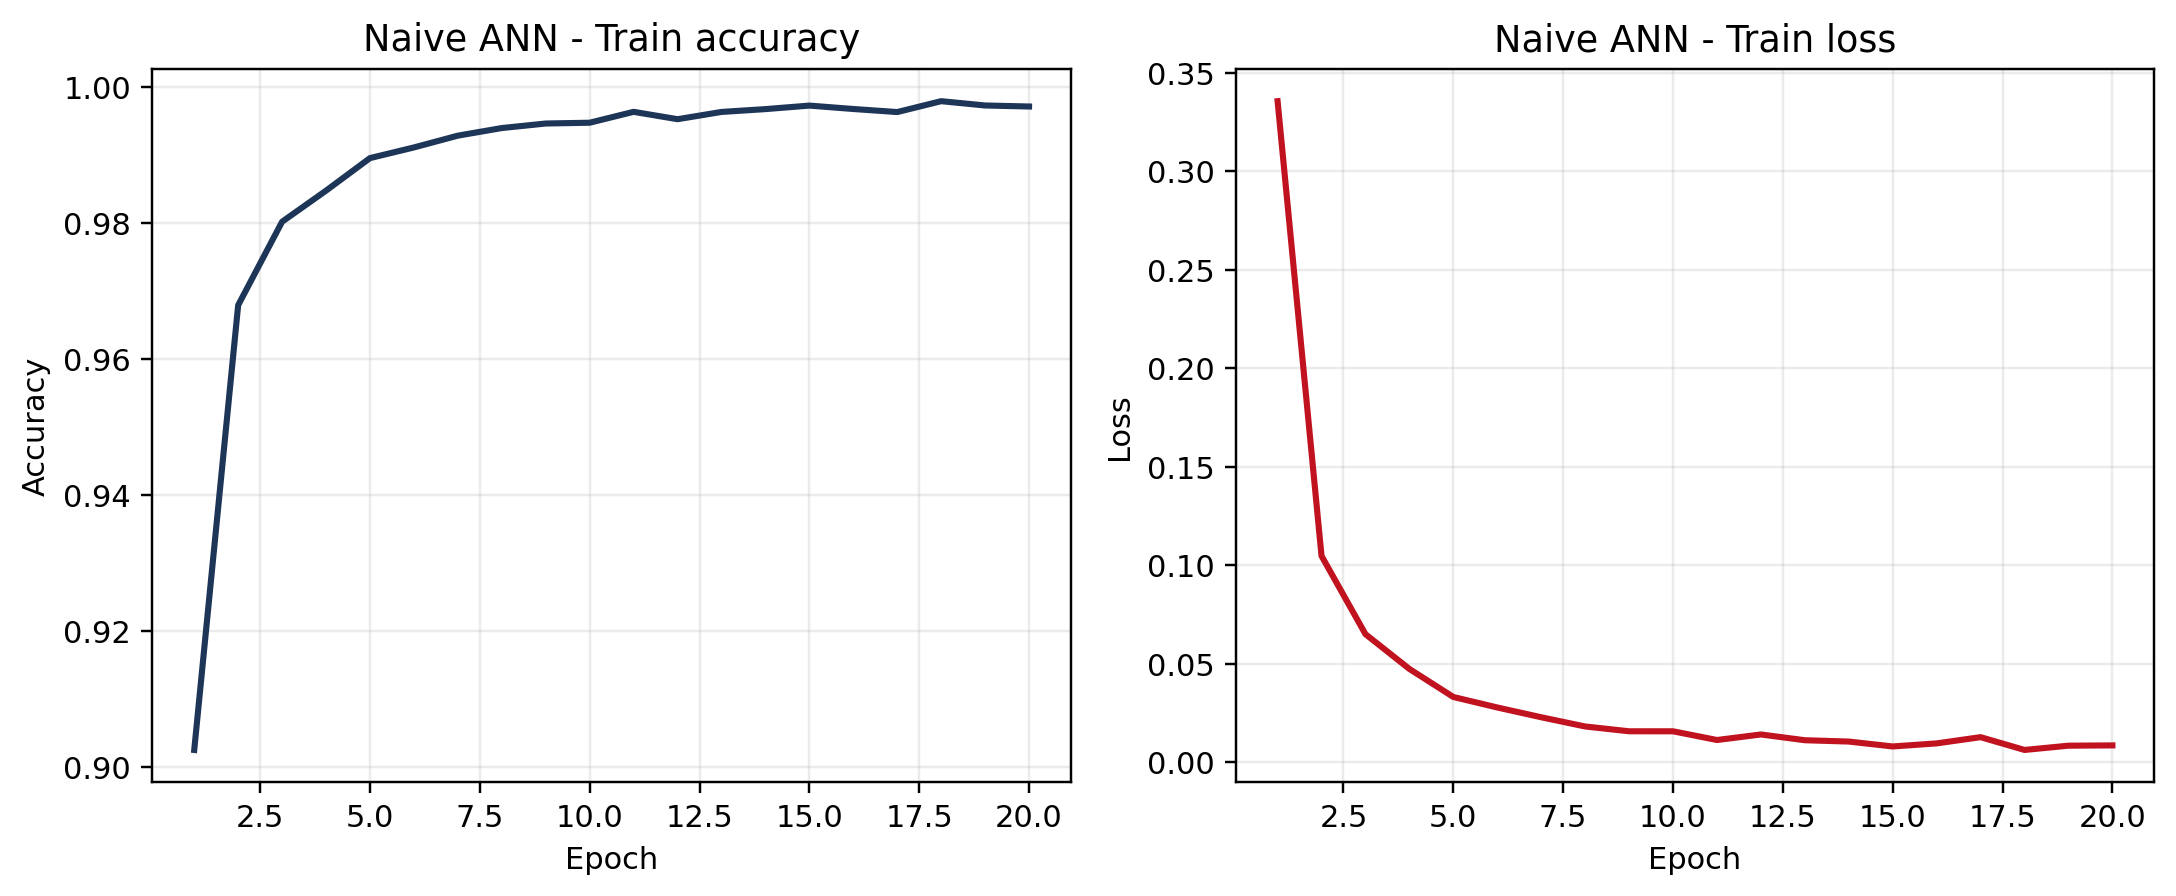
\includegraphics[width=0.92\textwidth]{figures/mnist-models/naive_training_curves.png}
  \caption{Diễn biến train accuracy và train loss của Naive ANN.}
  \label{fig:mnist-naive-training}
\end{figure}

\begin{figure}[H]
  \centering
  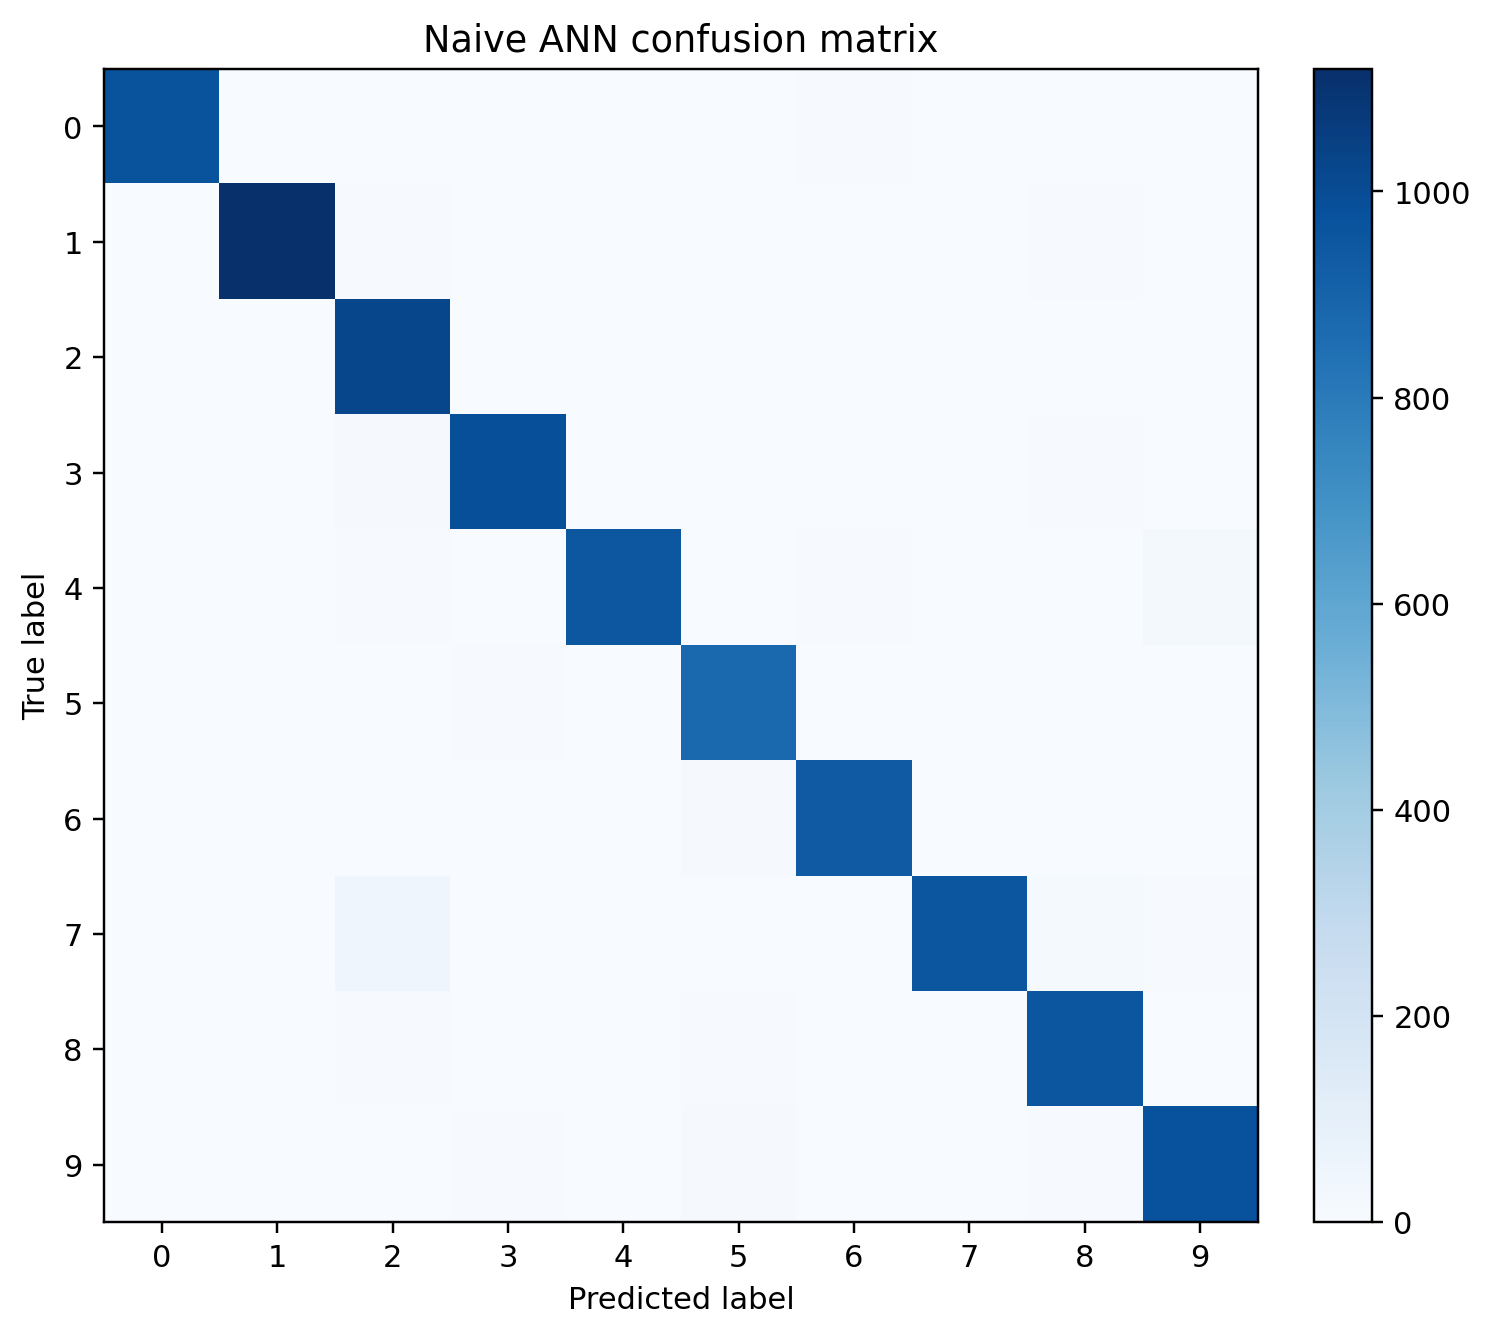
\includegraphics[width=0.72\textwidth]{figures/mnist-models/naive_confusion_matrix.png}
  \caption{Confusion matrix của Naive ANN trên tập test MNIST.}
  \label{fig:mnist-naive-confusion}
\end{figure}

\begin{figure}[H]
  \centering
  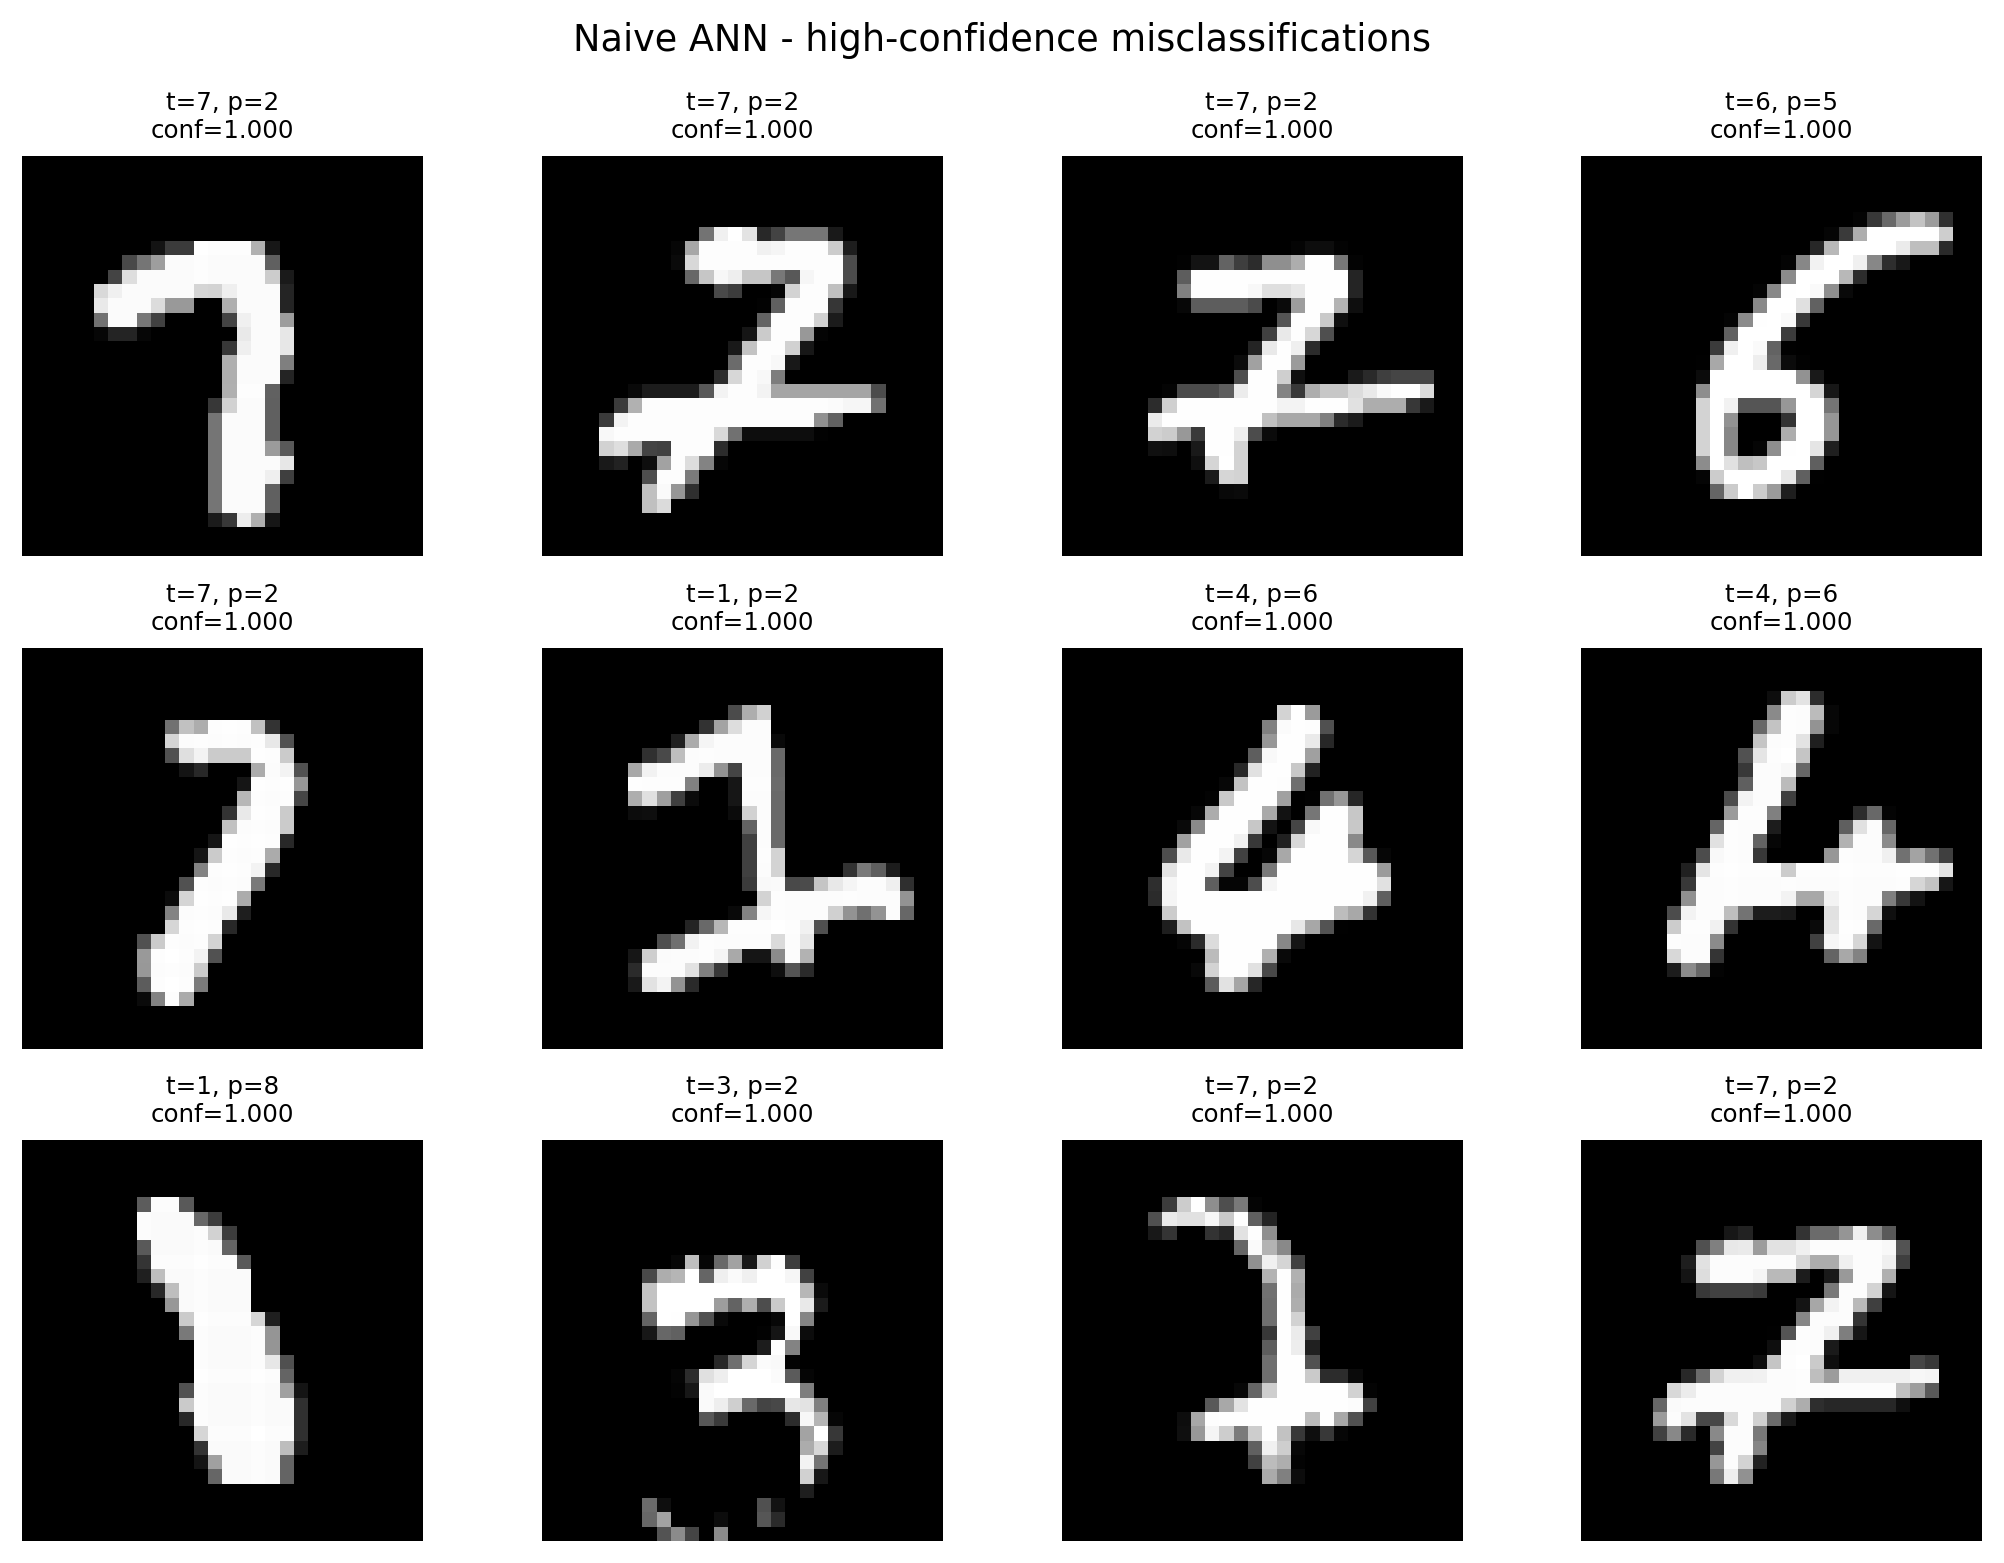
\includegraphics[width=0.92\textwidth]{figures/mnist-models/naive_misclassified_gallery.png}
  \caption{Một số mẫu test bị Naive ANN phân loại sai với độ tin cậy cao.}
  \label{fig:mnist-naive-gallery}
\end{figure}

\begin{figure}[H]
  \centering
  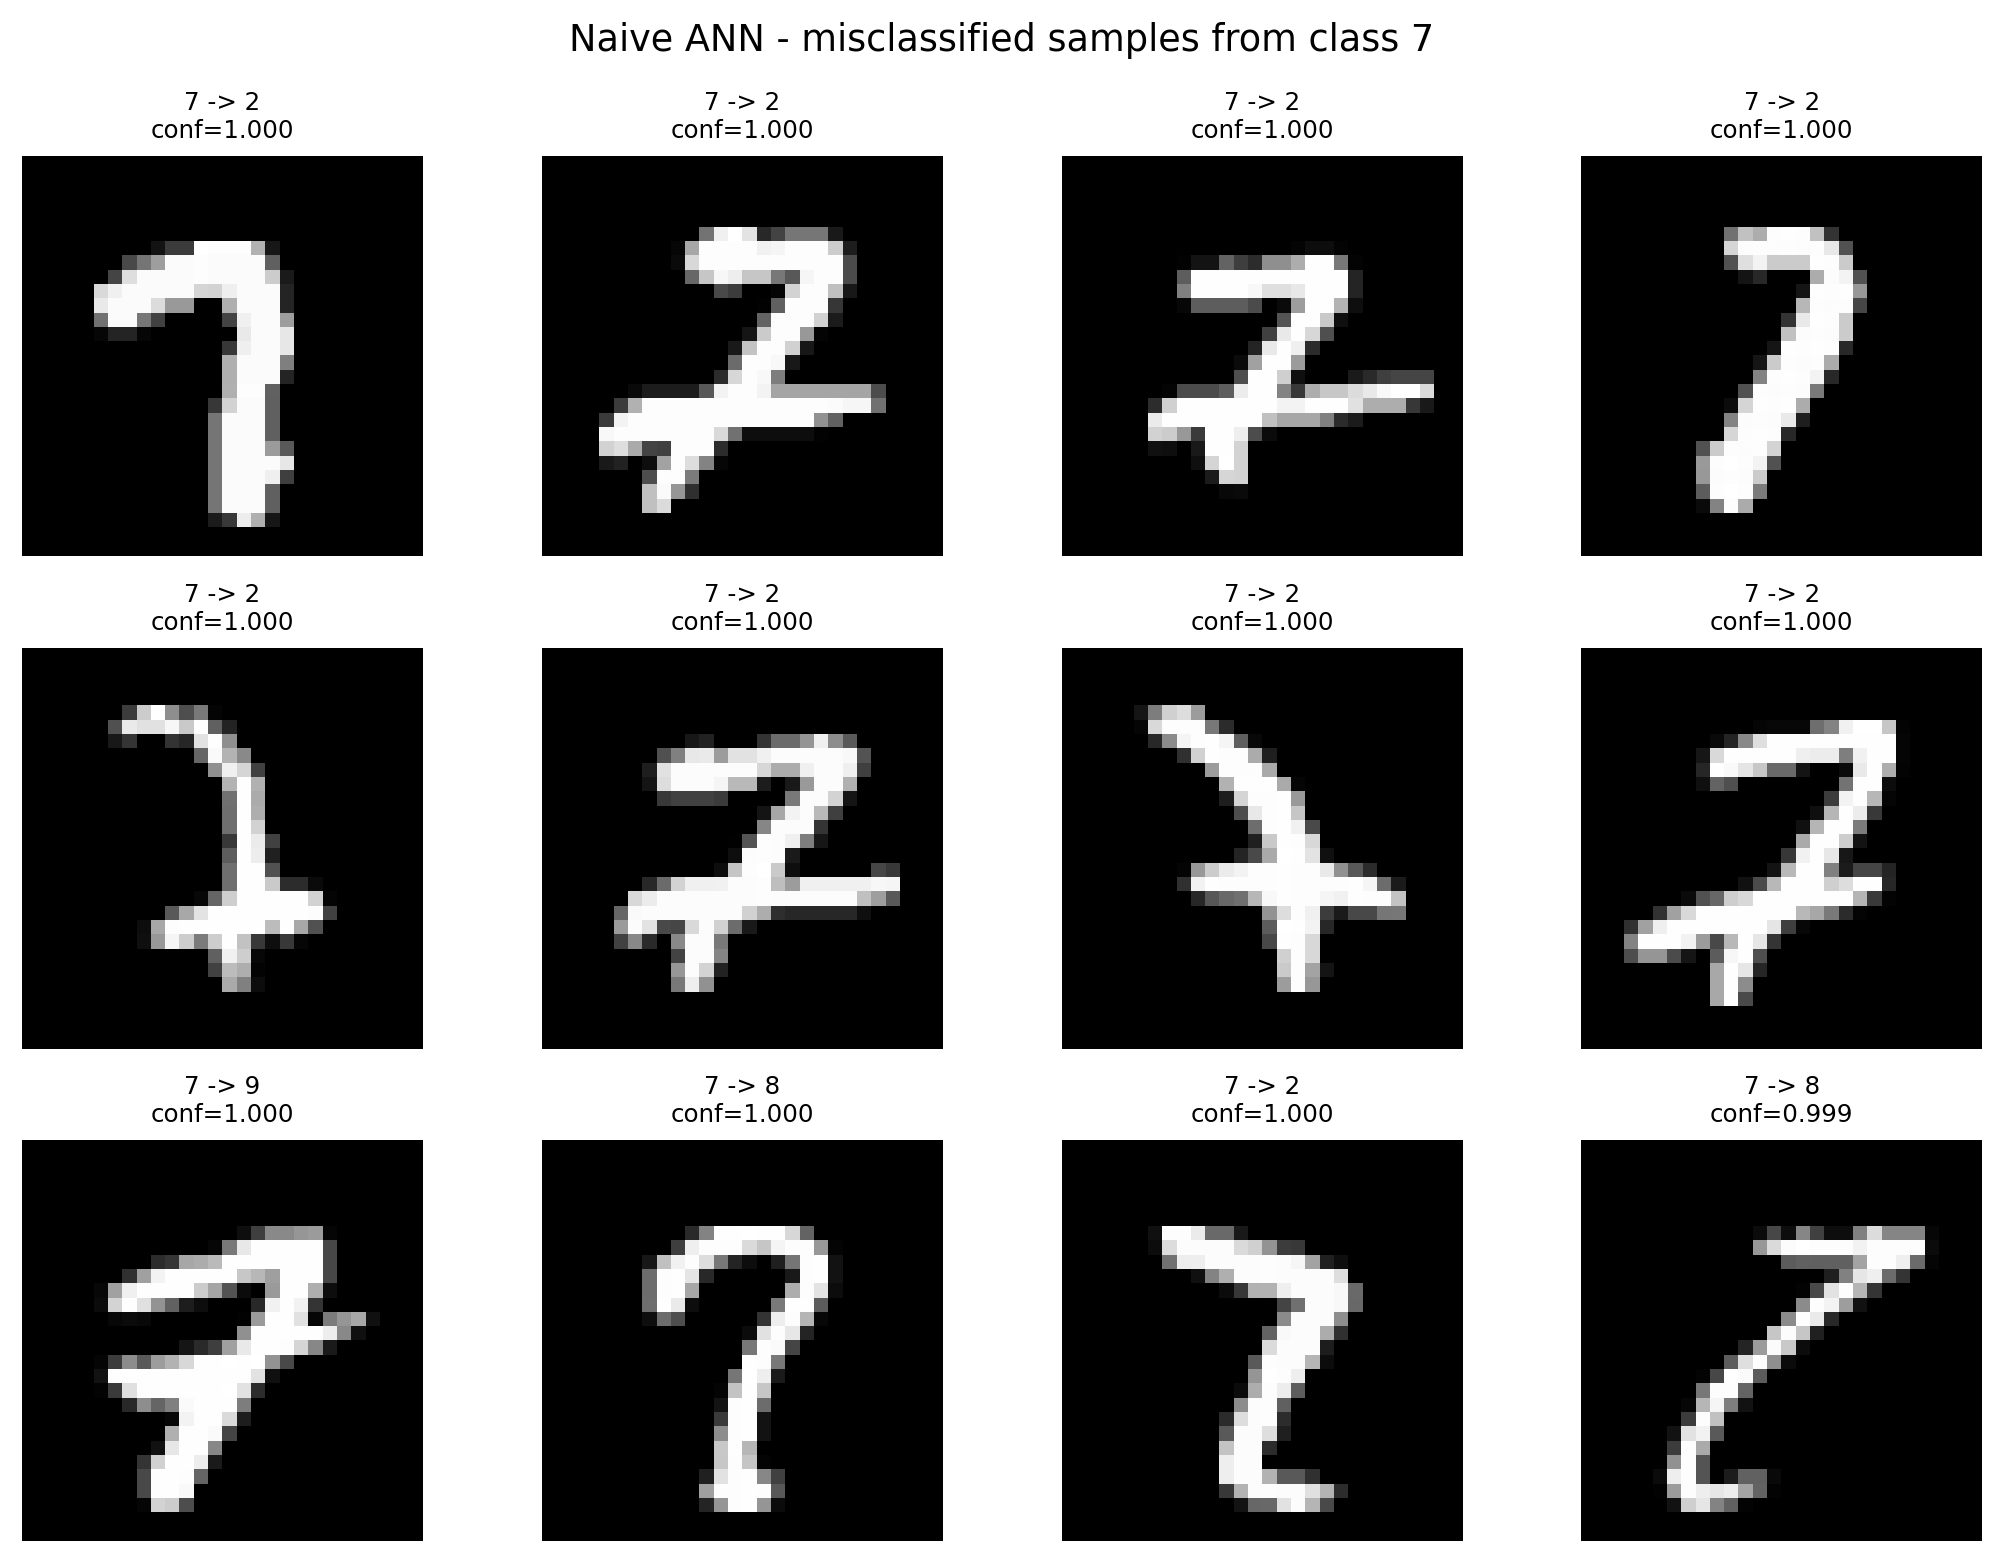
\includegraphics[width=0.92\textwidth]{figures/mnist-models/naive_class7_error_gallery.png}
  \caption{Các mẫu thuộc lớp $7$ bị Naive ANN phân loại sai.}
  \label{fig:mnist-naive-class7-gallery}
\end{figure}

\begin{table}[H]
\centering
\caption{Thống kê lỗi theo từng lớp của Naive ANN trên tập test MNIST}
\label{tab:mnist-naive-error-by-class}
\small
\begin{tabular}{c c c c c}
\toprule
Lớp thật & Số mẫu test & Số dự đoán sai & Tỉ lệ lỗi & Nhầm nhiều nhất \\
\midrule
0 & 980 & 11 & 1.12\% & $0 \rightarrow 6$ (7 mẫu) \\
1 & 1135 & 16 & 1.41\% & $1 \rightarrow 2$ (7 mẫu) \\
2 & 1032 & 13 & 1.26\% & $2 \rightarrow 0$ (2 mẫu) \\
3 & 1010 & 24 & 2.38\% & $3 \rightarrow 2$ (13 mẫu) \\
4 & 982 & 32 & 3.26\% & $4 \rightarrow 9$ (18 mẫu) \\
5 & 892 & 14 & 1.57\% & $5 \rightarrow 3$ (7 mẫu) \\
6 & 958 & 21 & 2.19\% & $6 \rightarrow 5$ (11 mẫu) \\
7 & 1028 & 71 & 6.91\% & $7 \rightarrow 2$ (44 mẫu) \\
8 & 974 & 18 & 1.85\% & $8 \rightarrow 5$ (6 mẫu) \\
9 & 1009 & 34 & 3.37\% & $9 \rightarrow 5$ (9 mẫu) \\
\bottomrule
\end{tabular}
\end{table}


Naive ANN đạt $97.46\%$ test accuracy và có \textit{generalization gap} khoảng $2.25\%$, lớn nhất trong bốn biến thể. Confusion matrix của mô hình cho thấy lỗi không phân bố ngẫu nhiên mà tập trung rất mạnh vào các cặp có hình thái gần nhau, nổi bật nhất là $7 \rightarrow 2$, $4 \rightarrow 9$, $3 \rightarrow 2$ và $6 \rightarrow 5$. Các lớp khó nhất là $7$, $9$ và $4$. Tập hợp các mẫu sai cũng cho thấy những ảnh bị nhầm thường có xu hướng nghiêng, lệch tâm hoặc có stroke chồng lấn về cấu trúc, đúng với insight từ EDA.

Bảng thống kê lỗi theo lớp ở ngay trên làm rõ hơn bản chất của các lỗi này. Lớp $7$ có tỉ lệ lỗi cao nhất, gần $7\%$, và riêng cặp $7 \rightarrow 2$ đã chiếm $44$ mẫu sai. Hai lớp $4$ và $9$ cũng có tỉ lệ lỗi cao vì chúng phụ thuộc mạnh vào vị trí giao nhau giữa các stroke và độ nghiêng của nét dọc. Hình hiển thị riêng cho lớp $7$ cho thấy rõ điểm chung của các mẫu bị nhầm: nét ngang phía trên thường ngắn hoặc cong, thân dọc bị nghiêng và phần chân dưới tạo thành một móc ngang, khiến hình tổng thể gần với số $2$; ở một số mẫu khác, phần đầu cong hơn và phần thân kéo dài xuống dưới khiến mô hình còn nhầm sang $8$ hoặc $9$. Nhóm lỗi $3 \rightarrow 2$, $4 \rightarrow 9$, $6 \rightarrow 5$, $7 \rightarrow 2$ và $9 \rightarrow 5$ đều có một đặc điểm chung: raw pixel giữ được cường độ sáng, nhưng biểu diễn rất kém thông tin về hướng nét và bố cục hình học.

Từ kết quả này, có thể thấy raw pixel phẳng là chưa đủ. Vấn đề không phải ANN không học được MNIST, mà là ANN đang phải tự học quá nhiều thông tin hình học và hướng nét từ biểu diễn đầu vào còn quá thô. Vì vậy, bước cải tiến kế tiếp hợp lý nhất là chuẩn hóa hình học bằng \textit{deslant + recenter} để giảm lệch tâm và độ nghiêng, đồng thời thêm HOG để đưa thông tin gradient vào mô hình ngay từ đầu. Nói cách khác, biến thể kế tiếp không được thiết kế ngẫu nhiên, mà được sinh ra trực tiếp từ đúng nhóm lỗi mà baseline vừa bộc lộ.

\subsection{Single-branch ANN}

Trong biến thể này, phần HOG cần được nêu rõ vì đây là nguồn tạo ra phần lớn thông tin hình học mới so với baseline. Với cấu hình \textit{orientations} $= 9$, \textit{pixels per cell} $= (4,4)$, \textit{cells per block} $= (2,2)$, ảnh $28 \times 28$ được chia thành lưới $7 \times 7$ cell. Khi block $2 \times 2$ trượt trên lưới này, số block theo mỗi chiều là $7 - 2 + 1 = 6$, nên tổng cộng có $6 \times 6 = 36$ block. Mỗi block chứa $2 \times 2$ cell và mỗi cell có $9$ bins hướng gradient, do đó một block sinh ra $2 \times 2 \times 9 = 36$ đặc trưng. Tổng số chiều HOG là $36 \times 36 = 1296$. Khi ghép với raw pixel $784$ chiều, đầu vào chung của single-branch trở thành vector $2080 = 784 + 1296$ chiều.
Single-branch ANN là bước cải tiến trực tiếp từ baseline. Ảnh trước hết được đưa qua \textit{deslant} để giảm biến thiên nghiêng và \textit{recenter} để đưa chữ số về vị trí ổn định hơn trong khung hình. Sau đó raw pixel $784$ chiều được giữ lại và ghép với vector HOG $1296$ chiều thành đầu vào chung $2080$ chiều. MLP phía sau có dạng $2080 \rightarrow 1024 \rightarrow 512 \rightarrow 256 \rightarrow 10$. Kích thước $1024$ ở tầng đầu được giữ đủ lớn để không làm mất thông tin khi raw pixel và HOG vừa mới được ghép lại, sau đó nén dần về $512$ rồi $256$ để đưa sang lớp phân loại cuối. BatchNorm được thêm để ổn định kích hoạt ở các tầng ẩn, còn Dropout được dùng để tăng regularization và giảm chênh lệch giữa train và test.

Nếu viết chặt chẽ hơn về vai trò của hai kỹ thuật này, BatchNorm và Dropout không giải quyết cùng một bài toán. BatchNorm chủ yếu giúp ổn định kích hoạt và làm quá trình tối ưu bớt nhạy với chênh lệch phân bố giữa các chiều đặc trưng, điều này đặc biệt quan trọng vì đầu vào $2080$ chiều được ghép từ raw pixel và HOG. Dropout thì nhắm vào regularization: nó buộc mạng không được phụ thuộc quá mạnh vào một nhóm neuron cụ thể trong lúc train. Ở đây, Dropout $(p=0.25)$ được đặt sau mỗi tầng ẩn để giảm độ nhạy của các lớp fully-connected có khá nhiều tham số. Nói ngắn gọn, BatchNorm chủ yếu nhắm về ổn định tối ưu và scale kích hoạt, còn Dropout nhắm về regularization; hai thứ được dùng đồng thời vì chúng bổ sung nhau thay vì thay thế nhau.

\begin{figure}[H]
  \centering
  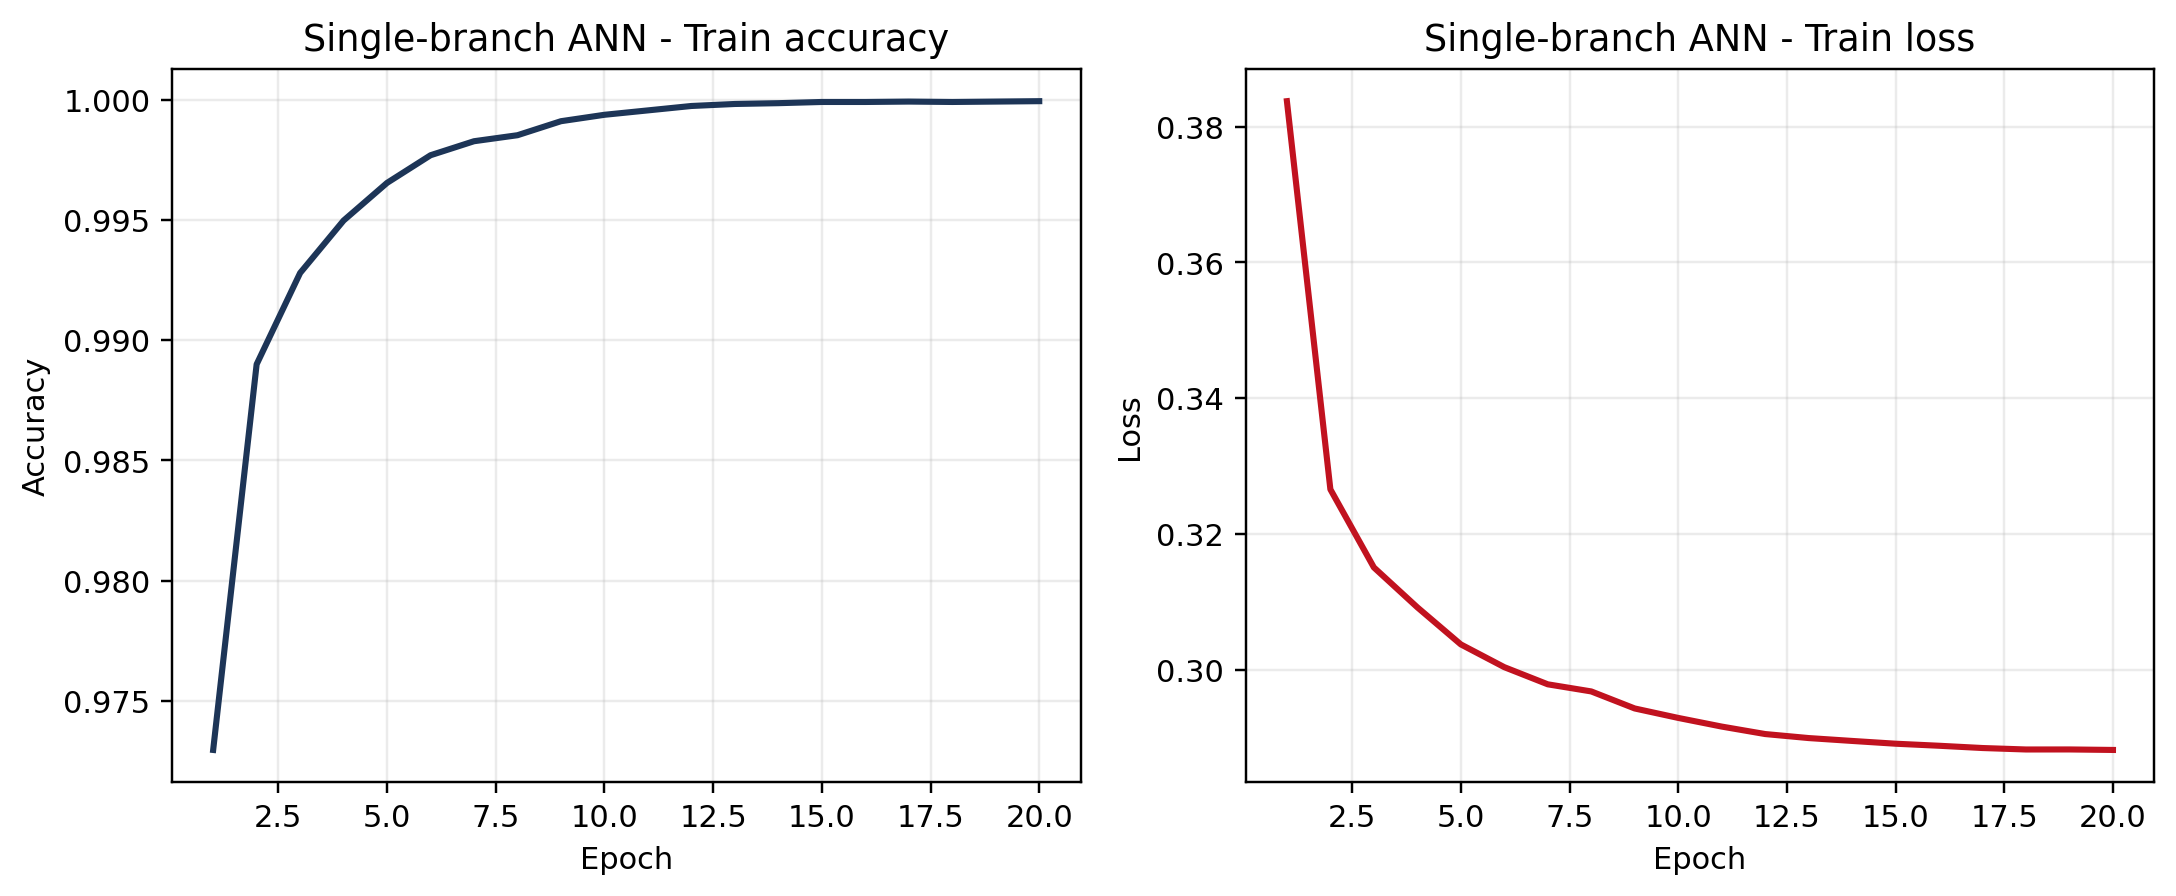
\includegraphics[width=0.92\textwidth]{figures/mnist-models/single_branch_training_curves.png}
  \caption{Diễn biến train accuracy và train loss của Single-branch ANN.}
  \label{fig:mnist-single-training}
\end{figure}

\begin{figure}[H]
  \centering
  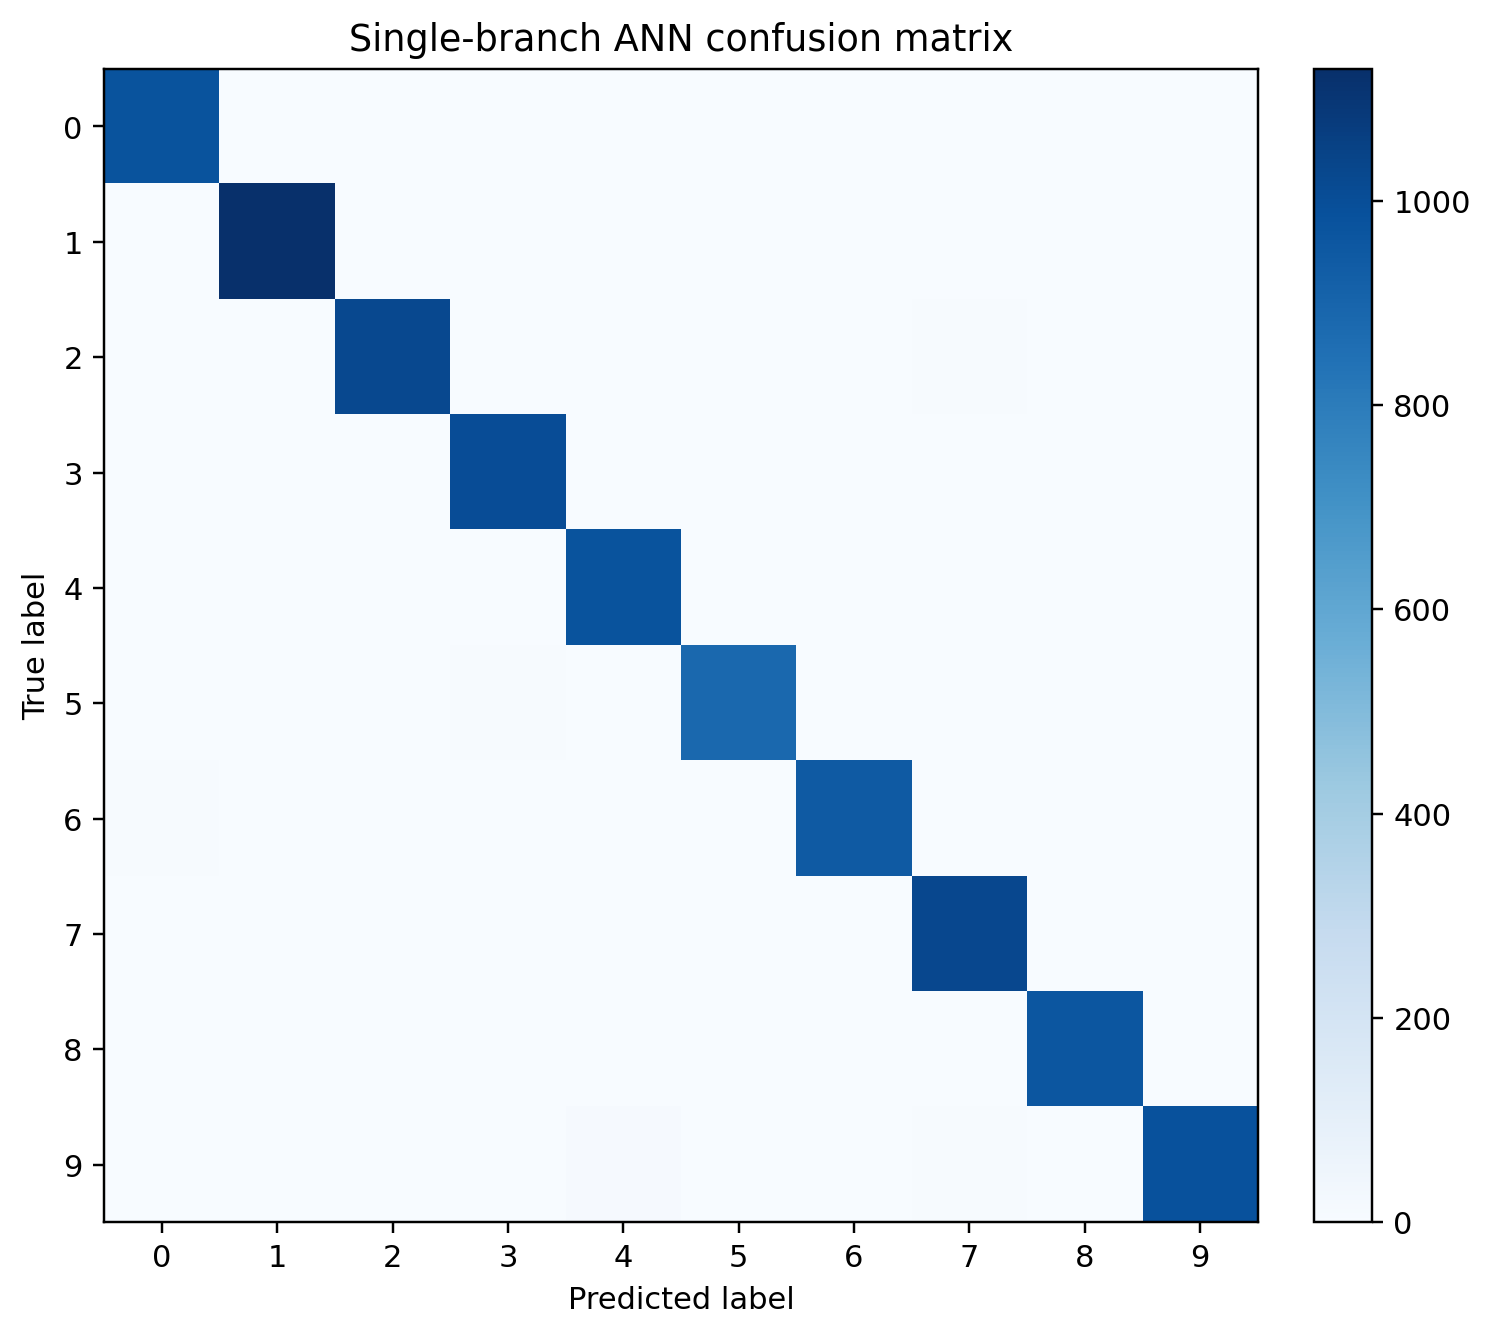
\includegraphics[width=0.72\textwidth]{figures/mnist-models/single_branch_confusion_matrix.png}
  \caption{Confusion matrix của Single-branch ANN trên tập test MNIST.}
  \label{fig:mnist-single-confusion}
\end{figure}

\begin{figure}[H]
  \centering
  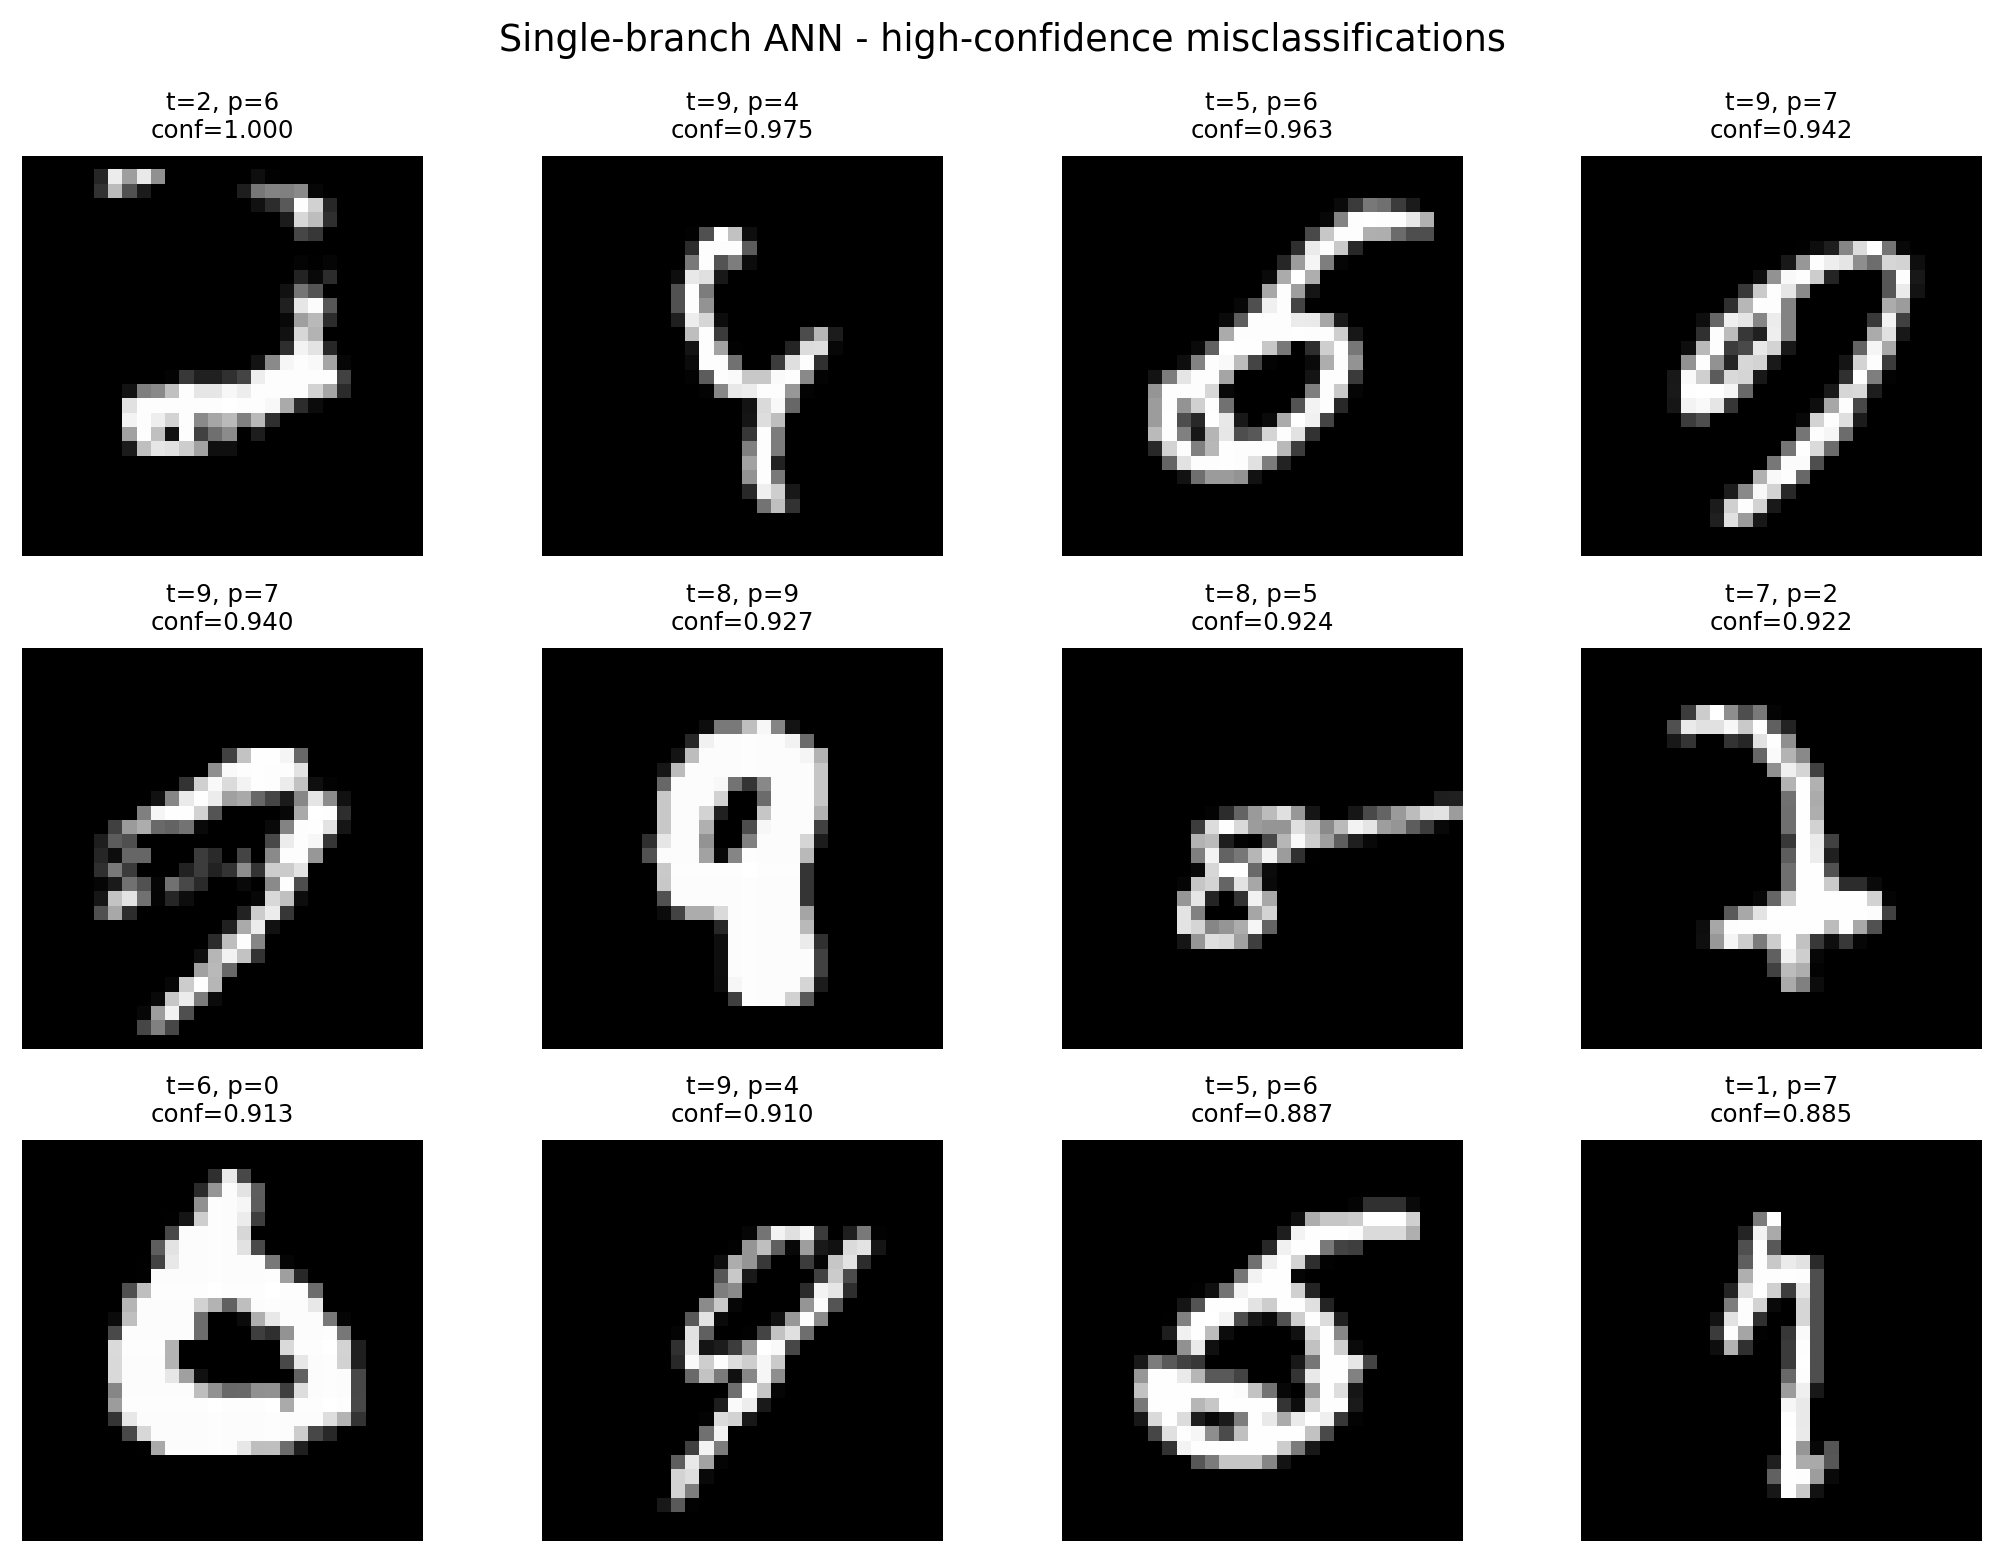
\includegraphics[width=0.92\textwidth]{figures/mnist-models/single_branch_misclassified_gallery.png}
  \caption{Một số mẫu test bị Single-branch ANN phân loại sai với độ tin cậy cao.}
  \label{fig:mnist-single-gallery}
\end{figure}

Single-branch ANN đạt $99.14\%$ test accuracy và giảm \textit{generalization gap} xuống khoảng $0.86\%$. Đây là bước nhảy lớn nhất trong toàn bộ quá trình thử nghiệm, cho thấy tiền xử lý và đặc trưng hóa giải quyết đúng nút thắt của baseline. Các cặp nhầm lẫn lớn nhất giảm mạnh; lỗi còn lại chủ yếu tập trung ở các chữ số $9$, $6$, $5$ và $8$, nổi bật nhất là $9 \rightarrow 4$ và $9 \rightarrow 7$. Gallery các mẫu sai cho thấy ảnh bị nhầm lúc này không còn lệch tâm hay nghiêng quá mạnh như baseline, mà chủ yếu khó ở mức hình thái stroke cục bộ.

Sau bước này, giả thuyết tự nhiên tiếp theo là: nếu các lỗi còn lại nằm ở chi tiết cục bộ của nét viết, có thể tăng thêm đa dạng nét viết trong tập train bằng augmentation cục bộ, thay vì tiếp tục thay đổi mạnh kiến trúc.

\subsection{Single-branch + local augmentation}

Biến thể này giữ nguyên kiến trúc single-branch và toàn bộ pipeline \textit{deslant + recenter + HOG + BatchNorm + Dropout}, nhưng bổ sung thêm augmentation cục bộ. Thay vì tăng mạnh các phép affine toàn cục, mô hình chỉ thêm \textit{elastic distortion} nhẹ để mô phỏng độ cong cục bộ của nét viết và \textit{stroke jitter} nhẹ để mô phỏng thay đổi bề dày nét. Ý tưởng của biến thể này là sau khi \textit{deslant} và \textit{recenter} đã xử lý phần lớn biến thiên hình học toàn cục, augmentation nên tập trung vào phần biến thiên nét viết mà tiền xử lý chưa giải quyết hết.

\begin{figure}[H]
  \centering
  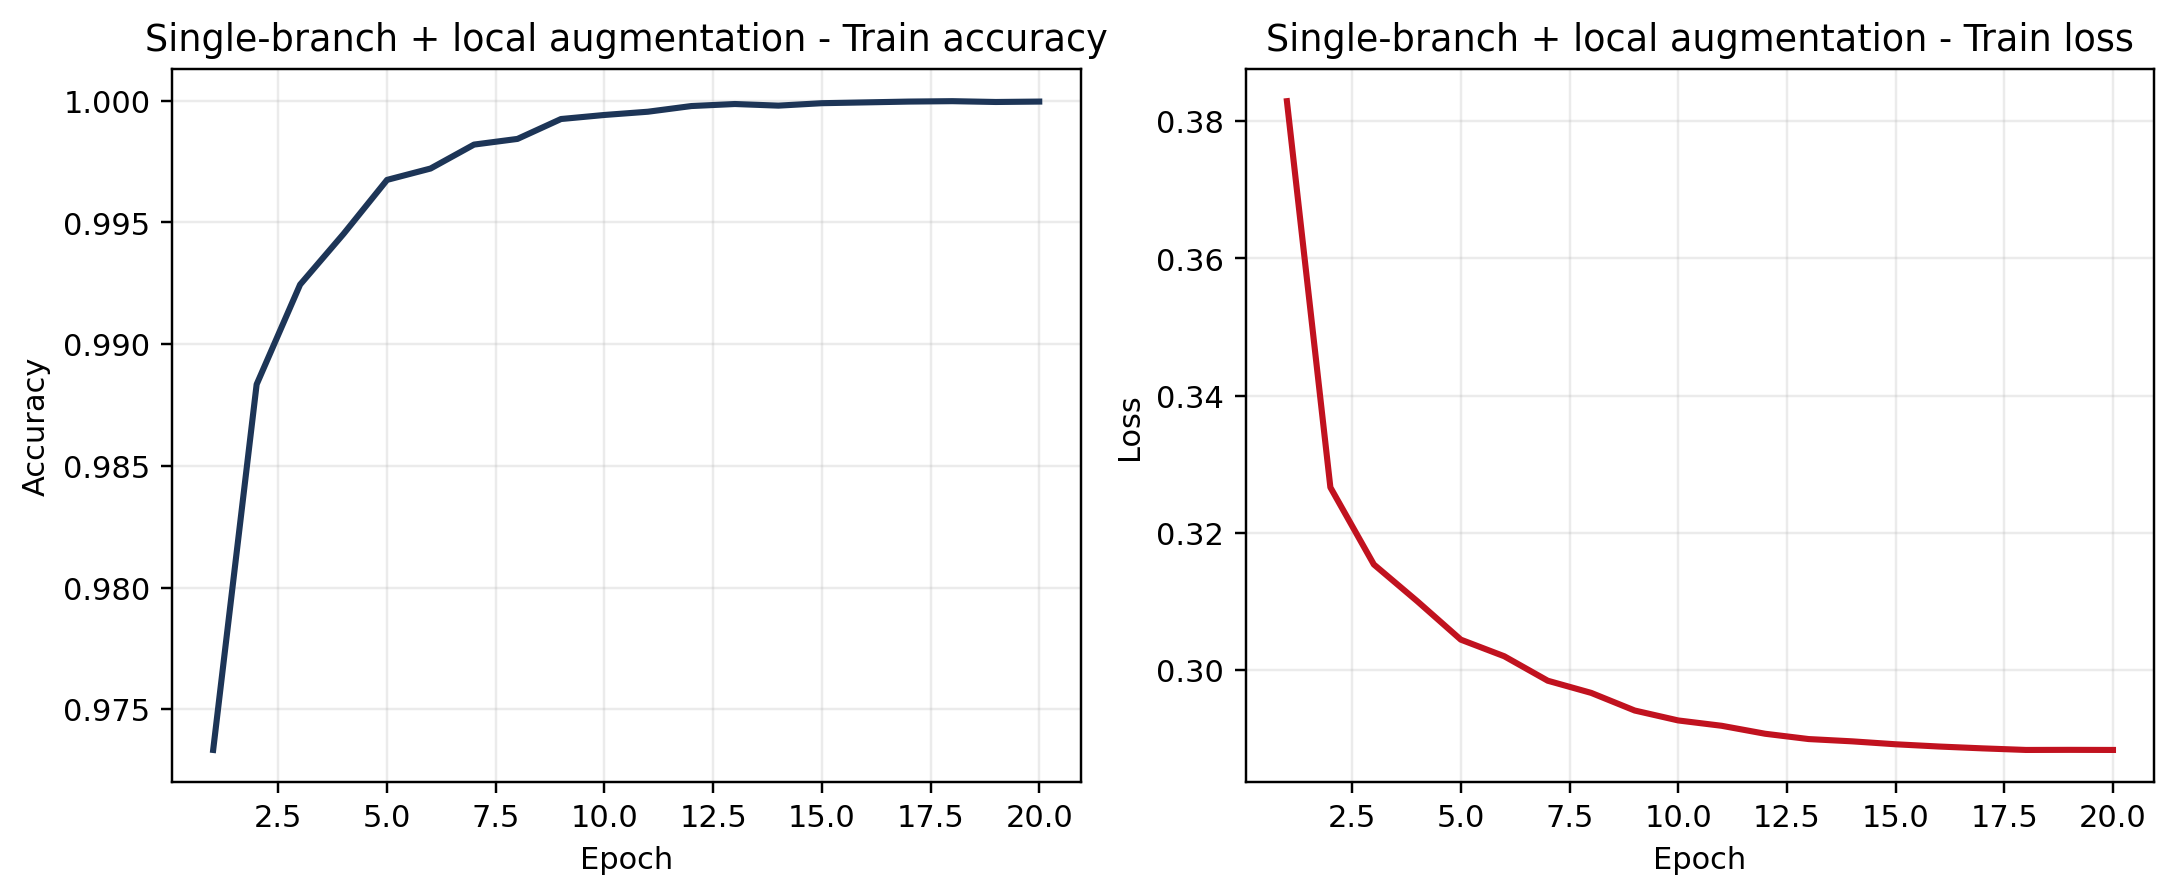
\includegraphics[width=0.92\textwidth]{figures/mnist-models/single_branch_augmented_training_curves.png}
  \caption{Diễn biến train accuracy và train loss của Single-branch ANN với local augmentation.}
  \label{fig:mnist-single-aug-training}
\end{figure}

\begin{figure}[H]
  \centering
  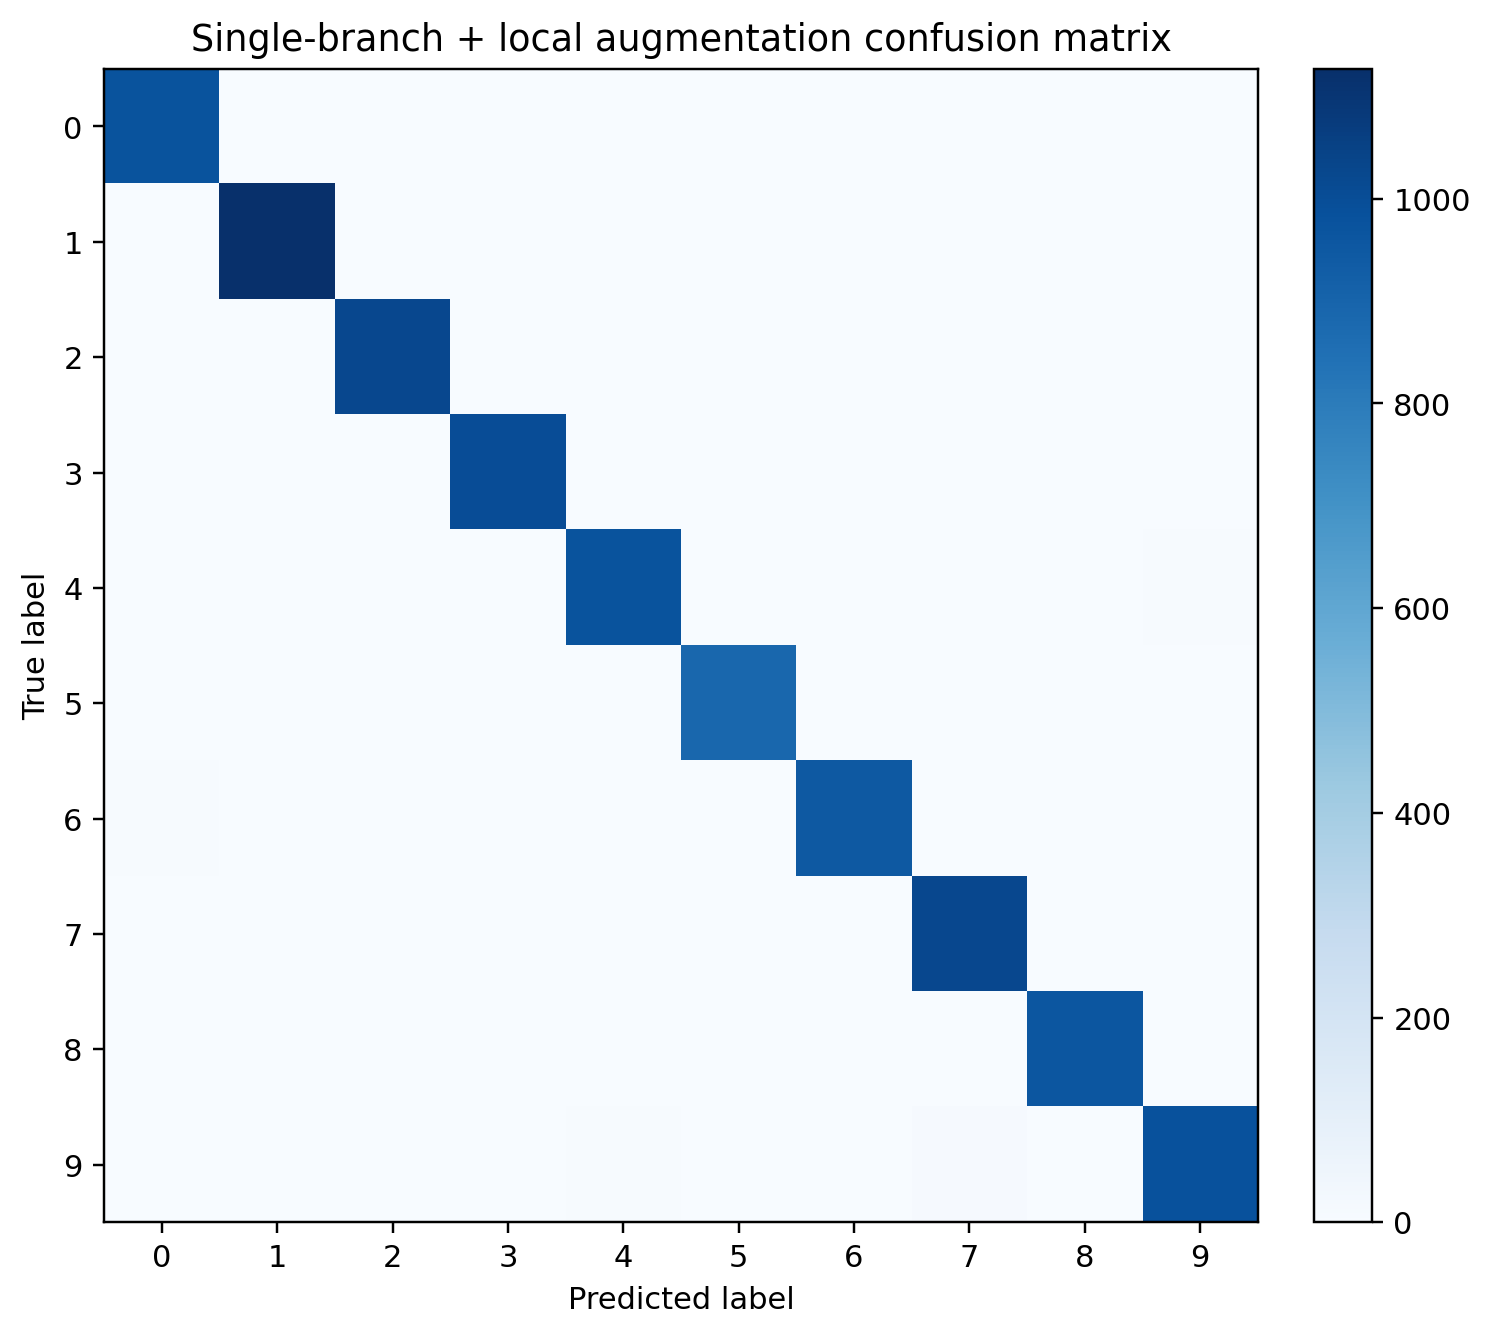
\includegraphics[width=0.72\textwidth]{figures/mnist-models/single_branch_augmented_confusion_matrix.png}
  \caption{Confusion matrix của Single-branch ANN với local augmentation trên tập test MNIST.}
  \label{fig:mnist-single-aug-confusion}
\end{figure}

\begin{figure}[H]
  \centering
  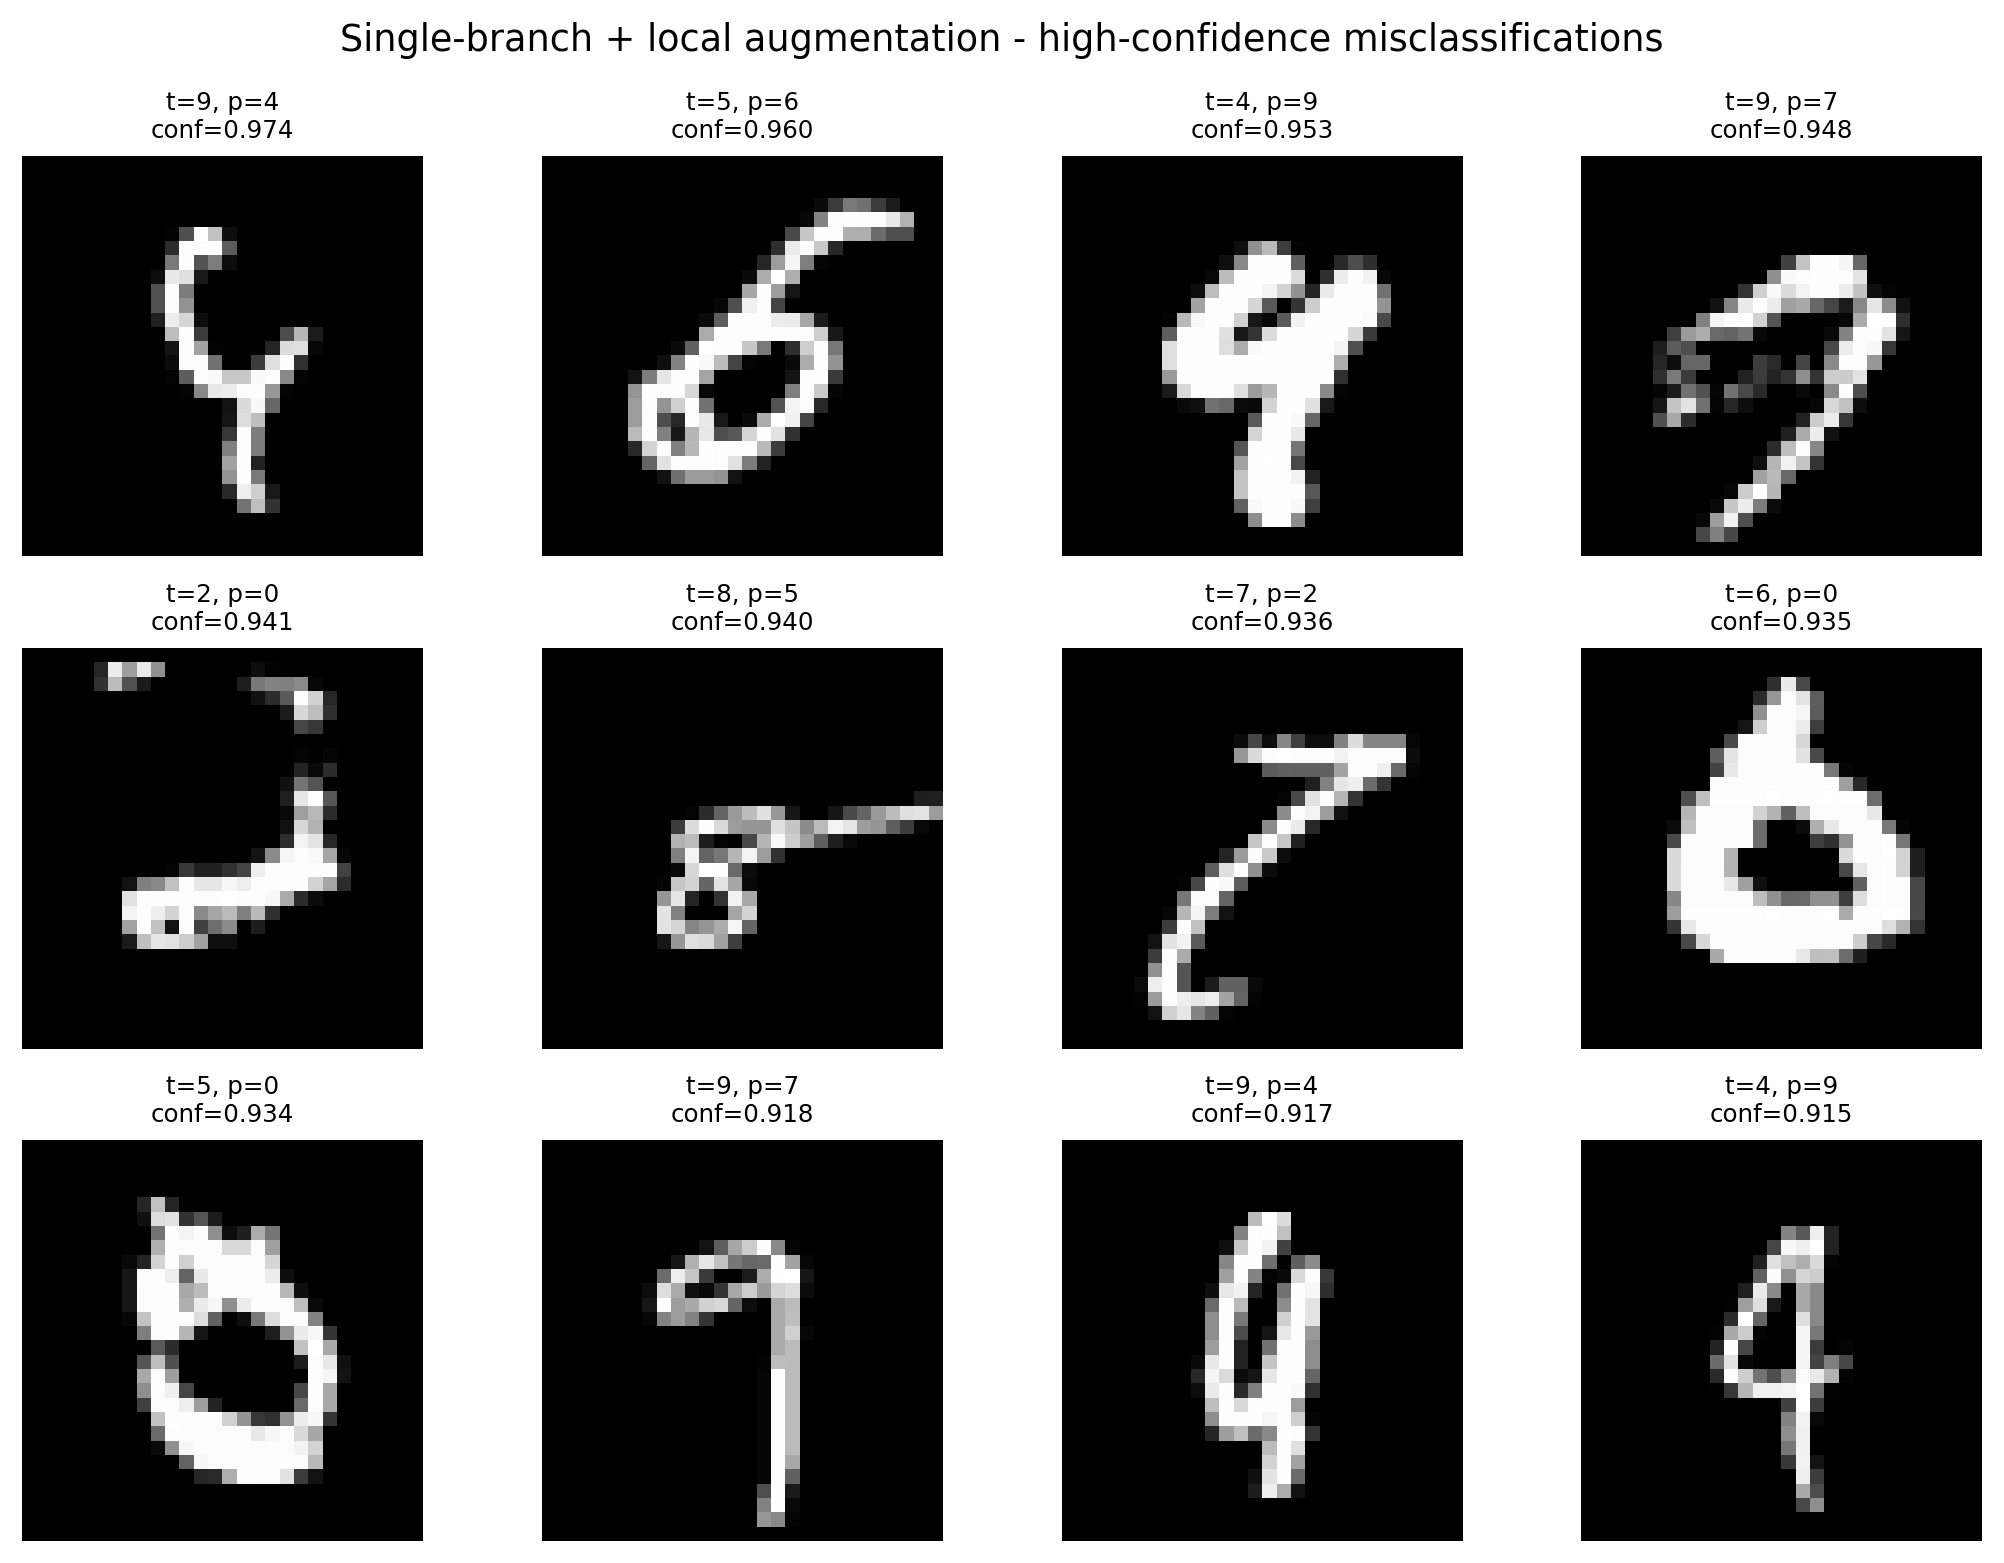
\includegraphics[width=0.92\textwidth]{figures/mnist-models/single_branch_augmented_misclassified_gallery.png}
  \caption{Một số mẫu test bị Single-branch ANN với local augmentation phân loại sai.}
  \label{fig:mnist-single-aug-gallery}
\end{figure}

Biến thể này đạt $99.11\%$ test accuracy, gần như tương đương với single-branch gốc nhưng không vượt lên trên. Các lỗi lớn nhất vẫn xoay quanh chữ số $9$, đặc biệt là $9 \rightarrow 7$ và $9 \rightarrow 4$, trong khi lớp khó nhất vẫn là $9$ rồi tới $6$ và $8$. Nói cách khác, augmentation cục bộ làm mô hình bền hơn với biến thiên nét viết, nhưng không tạo ra bước nhảy mới về mặt tổng thể.

Từ đây xuất hiện một giả thuyết khác: có thể bottleneck không còn nằm ở độ đa dạng dữ liệu nữa, mà nằm ở cách raw pixel và HOG đang bị ghép quá sớm thành một vector chung. Nếu đúng vậy, nên thử cho mỗi loại đầu vào đi qua một nhánh riêng trước khi hợp nhất ở tầng sâu hơn.

\subsection{Two-branch ANN}

Two-branch ANN dùng cùng đầu vào và cùng pipeline tiền xử lý như single-branch, nhưng thay vì ghép raw pixel và HOG ngay từ đầu, mô hình tách chúng thành hai nhánh học riêng. Nhánh raw có dạng $784 \rightarrow 512 \rightarrow 256$, còn nhánh HOG có dạng $1296 \rightarrow 768 \rightarrow 256$. Nhánh HOG được cấp tầng đầu rộng hơn vì đầu vào của nó có số chiều lớn hơn và mang nhiều thông tin cấu trúc hơn raw pixel. Sau khi mỗi nhánh đã nén về $256$ chiều, hai vector được ghép lại thành $512$ chiều rồi đi qua head cuối $512 \rightarrow 256 \rightarrow 10$. Thiết kế này giúp mô hình học riêng hai kiểu biểu diễn trước khi hợp nhất chúng ở tầng sâu hơn.

\begin{figure}[H]
  \centering
  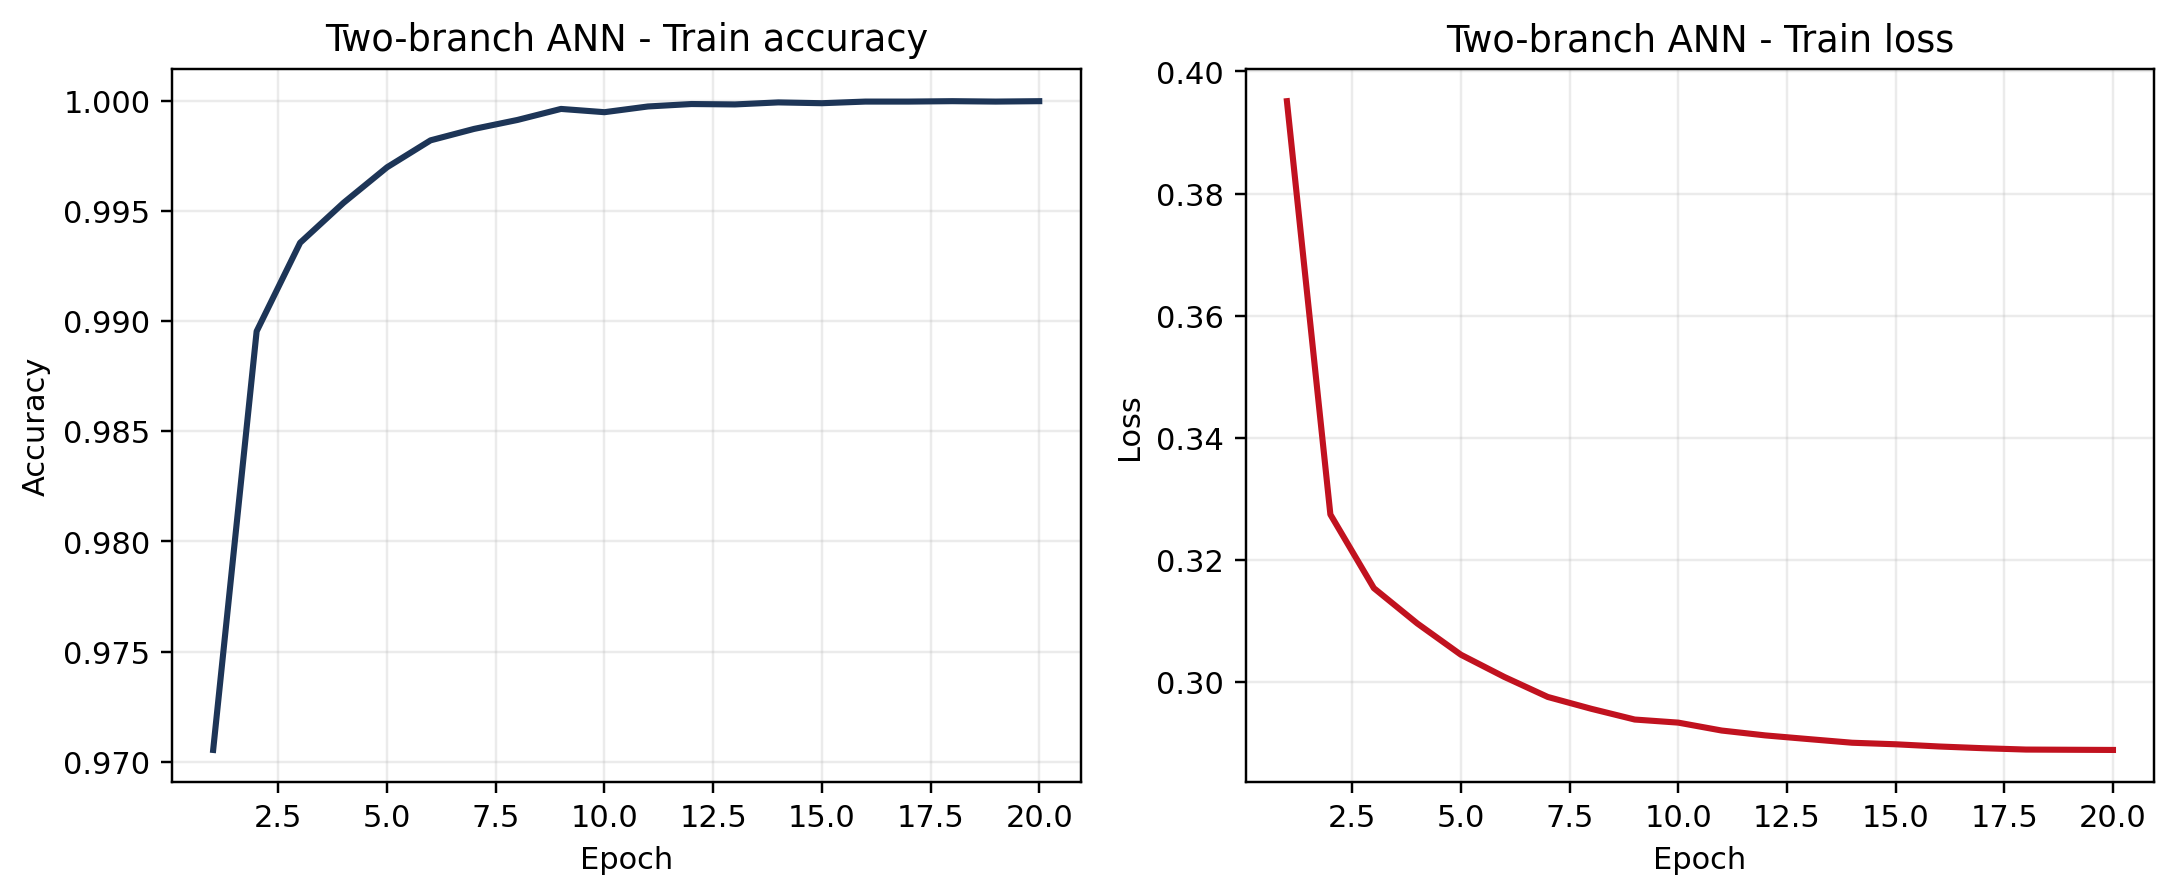
\includegraphics[width=0.92\textwidth]{figures/mnist-models/two_branch_training_curves.png}
  \caption{Diễn biến train accuracy và train loss của Two-branch ANN.}
  \label{fig:mnist-two-training}
\end{figure}

\begin{figure}[H]
  \centering
  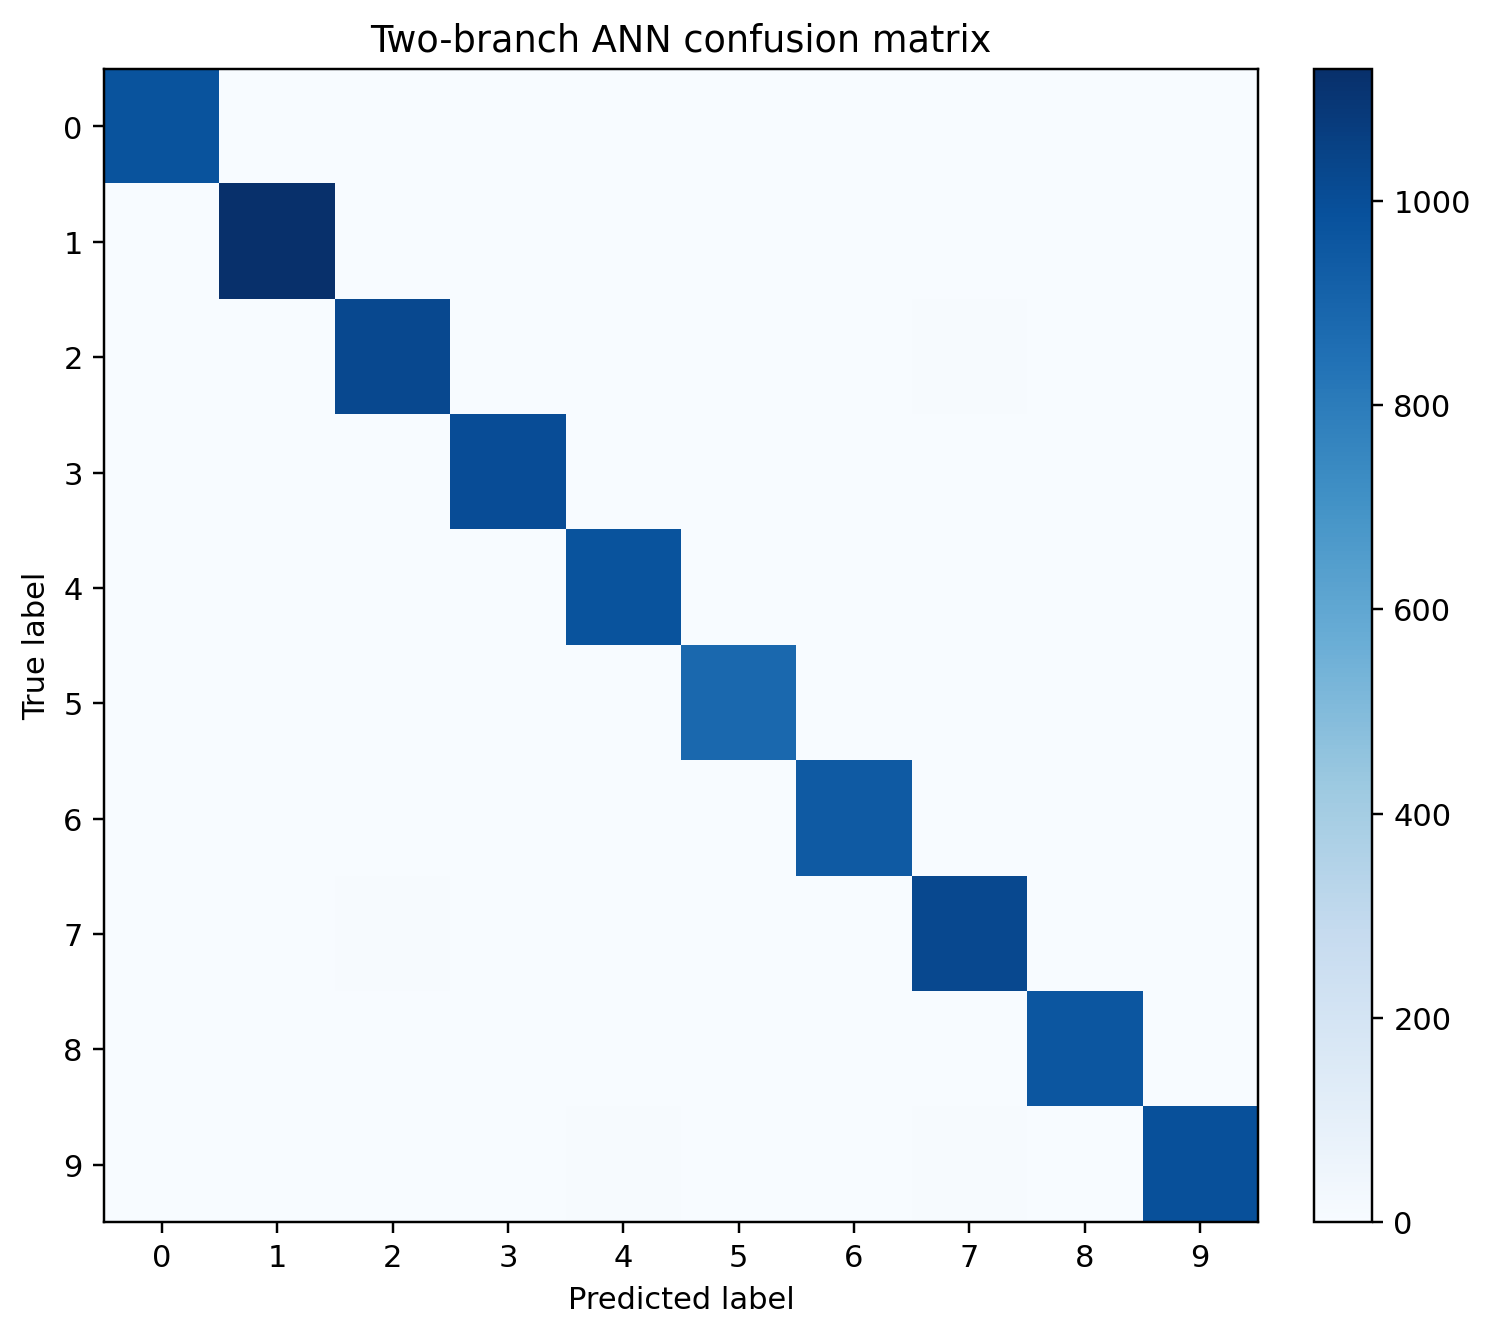
\includegraphics[width=0.72\textwidth]{figures/mnist-models/two_branch_confusion_matrix.png}
  \caption{Confusion matrix của Two-branch ANN trên tập test MNIST.}
  \label{fig:mnist-two-confusion}
\end{figure}

\begin{figure}[H]
  \centering
  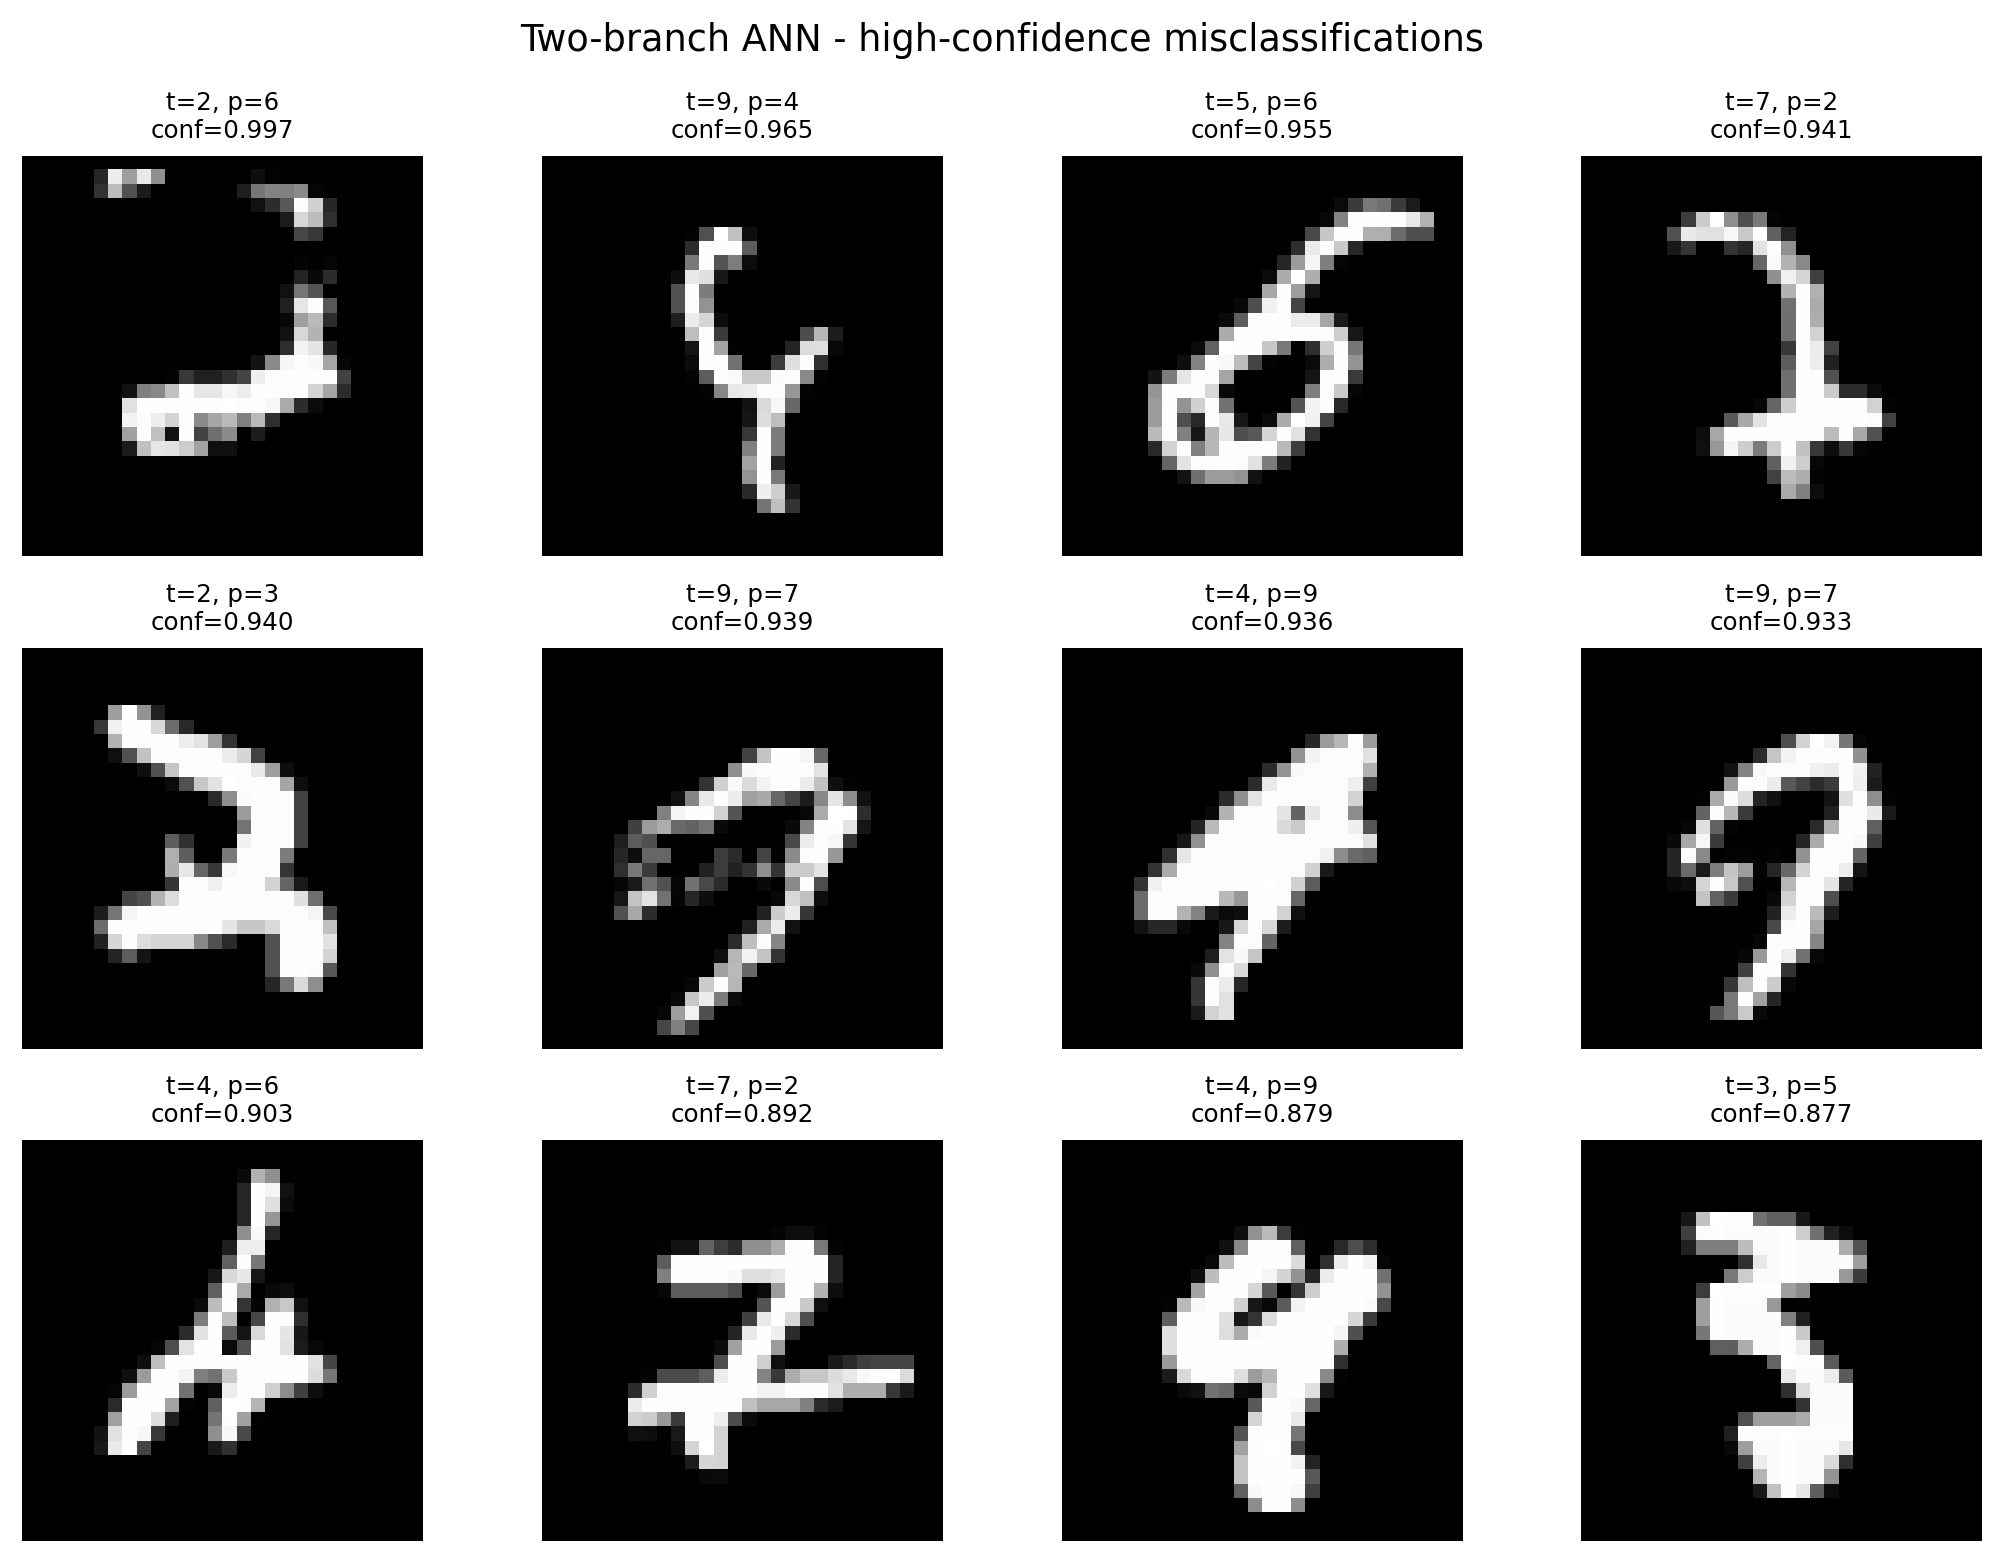
\includegraphics[width=0.92\textwidth]{figures/mnist-models/two_branch_misclassified_gallery.png}
  \caption{Một số mẫu test bị Two-branch ANN phân loại sai với độ tin cậy cao.}
  \label{fig:mnist-two-gallery}
\end{figure}

Two-branch ANN đạt $99.10\%$ test accuracy và có \textit{generalization gap} khoảng $0.90\%$. Kết quả này vẫn rất mạnh, nhưng không vượt được single-branch gốc trong lượt chạy hiện tại. Lỗi còn lại vẫn tập trung ở các cặp hình thái khó như $9 \rightarrow 4$, $9 \rightarrow 7$, $7 \leftrightarrow 2$ và $5 \rightarrow 3$. Điều này cho thấy giả thuyết “tách hai nhánh sẽ luôn tốt hơn” không phải lúc nào cũng đúng; sau khi dữ liệu đã được chuẩn hóa hình học tốt và HOG đã đủ mạnh, bottleneck còn lại không nhất thiết nằm ở kiến trúc hợp nhất đặc trưng.

\section{Tổng hợp kết quả và nhận xét}

\begin{table}[H]
\centering
\caption{Thông số đầu vào và kiến trúc của bốn biến thể ANN}
\label{tab:mnist-ann-architecture-details}
\small
\begin{tabularx}{\textwidth}{>{\raggedright\arraybackslash}p{2.8cm} >{\raggedright\arraybackslash}p{2.8cm} >{\raggedright\arraybackslash}X >{\raggedright\arraybackslash}p{3.0cm}}
\toprule
Biến thể & Đầu vào & Kiến trúc tuyến tính & Thành phần đi kèm \\
\midrule
Naive ANN & $784$ raw & $784 \rightarrow 1024 \rightarrow 512 \rightarrow 256 \rightarrow 10$ & ReLU only \\
Single-branch ANN & $2080 = 784 + 1296$ & $2080 \rightarrow 1024 \rightarrow 512 \rightarrow 256 \rightarrow 10$ & BN + GELU + Dropout$(0.25)$ \\
Single-branch + local augmentation & $2080 = 784 + 1296$ & $2080 \rightarrow 1024 \rightarrow 512 \rightarrow 256 \rightarrow 10$ & Same as single-branch \\
Two-branch ANN & Raw $784$, HOG $1296$ & Raw: $784 \rightarrow 512 \rightarrow 256$; HOG: $1296 \rightarrow 768 \rightarrow 256$; head: $512 \rightarrow 256 \rightarrow 10$ & BN + GELU + Dropout$(0.25)$ \\
\bottomrule
\end{tabularx}
\end{table}

\begin{table}[H]
\centering
\caption{Thông số huấn luyện và augmentation của bốn biến thể ANN}
\label{tab:mnist-ann-hyperparameters}
\small
\begin{tabularx}{\textwidth}{>{\raggedright\arraybackslash}p{2.8cm} >{\raggedright\arraybackslash}p{2.8cm} >{\raggedright\arraybackslash}p{2.4cm} >{\raggedright\arraybackslash}X}
\toprule
Biến thể & Tối ưu hóa & Batch/epoch & Tiền xử lý và augmentation lúc train \\
\midrule
Naive ANN & Adam, CE, $lr=10^{-3}$ & $256 / 20$ & Không tiền xử lý, không augmentation \\
Single-branch ANN & AdamW, CE+LS, cosine, $wd=10^{-4}$ & $256 / 20$ & Affine; deslant; recenter; HOG \\
Single-branch + local augmentation & AdamW, CE+LS, cosine, $wd=10^{-4}$ & $256 / 20$ & Affine nhẹ; elastic distortion; stroke jitter; deslant; recenter; HOG \\
Two-branch ANN & AdamW, CE+LS, cosine, $wd=10^{-4}$ & $256 / 20$ & Affine; deslant; recenter; tách raw/HOG \\
\bottomrule
\end{tabularx}
\end{table}


\begin{table}[H]
\centering
\caption{Logic chuyển từ một biến thể ANN sang biến thể kế tiếp trên MNIST}
\label{tab:mnist-ann-iteration-logic}
\small
\begin{tabularx}{\textwidth}{>{\raggedright\arraybackslash}p{2.7cm} >{\raggedright\arraybackslash}X >{\raggedright\arraybackslash}X}
\toprule
Biến thể hiện tại & Điểm yếu quan sát được & Ý tưởng cho biến thể kế tiếp \\
\midrule
Naive ANN & Generalization gap lớn; nhầm mạnh ở các cặp gần nhau như $7 \rightarrow 2$, $4 \rightarrow 9$ & Thêm \textit{deslant + recenter + HOG} để đưa thông tin hình học và hướng nét vào ANN \\
Single-branch ANN & Độ chính xác tăng mạnh nhưng vẫn nhạy với biến thiên nét viết cục bộ & Bổ sung \textit{elastic distortion} và \textit{stroke jitter} augmentation \\
Single-branch + local augmentation & Kết quả gần bão hòa; raw và HOG có thể đang bị hòa trộn quá sớm & Tách raw pixel và HOG thành hai nhánh riêng trước khi hợp nhất \\
\bottomrule
\end{tabularx}
\end{table}

\begin{table}[H]
\centering
\caption{So sánh bốn biến thể ANN trên MNIST Handwritten}
\label{tab:mnist-ann-model-comparison}
\begin{tabular}{l c c c}
\toprule
Mô hình & Final train acc & Test acc & Generalization gap \\
\midrule
Naive ANN & 0.9971 & 0.9746 & 0.0225 \\
Single-branch ANN & 1.0000 & 0.9914 & 0.0086 \\
Single-branch + local augmentation & 1.0000 & 0.9911 & 0.0089 \\
Two-branch ANN & 1.0000 & 0.9910 & 0.0090 \\
\bottomrule
\end{tabular}
\end{table}


\begin{figure}[H]
  \centering
  
\includegraphics[width=0.86\textwidth]{figures/mnist-models/model_comparison.png}
  \caption{So sánh test accuracy và generalization gap của bốn biến thể ANN trên MNIST.}
  \label{fig:mnist-model-comparison}
\end{figure}

\begin{figure}[H]
  \centering
  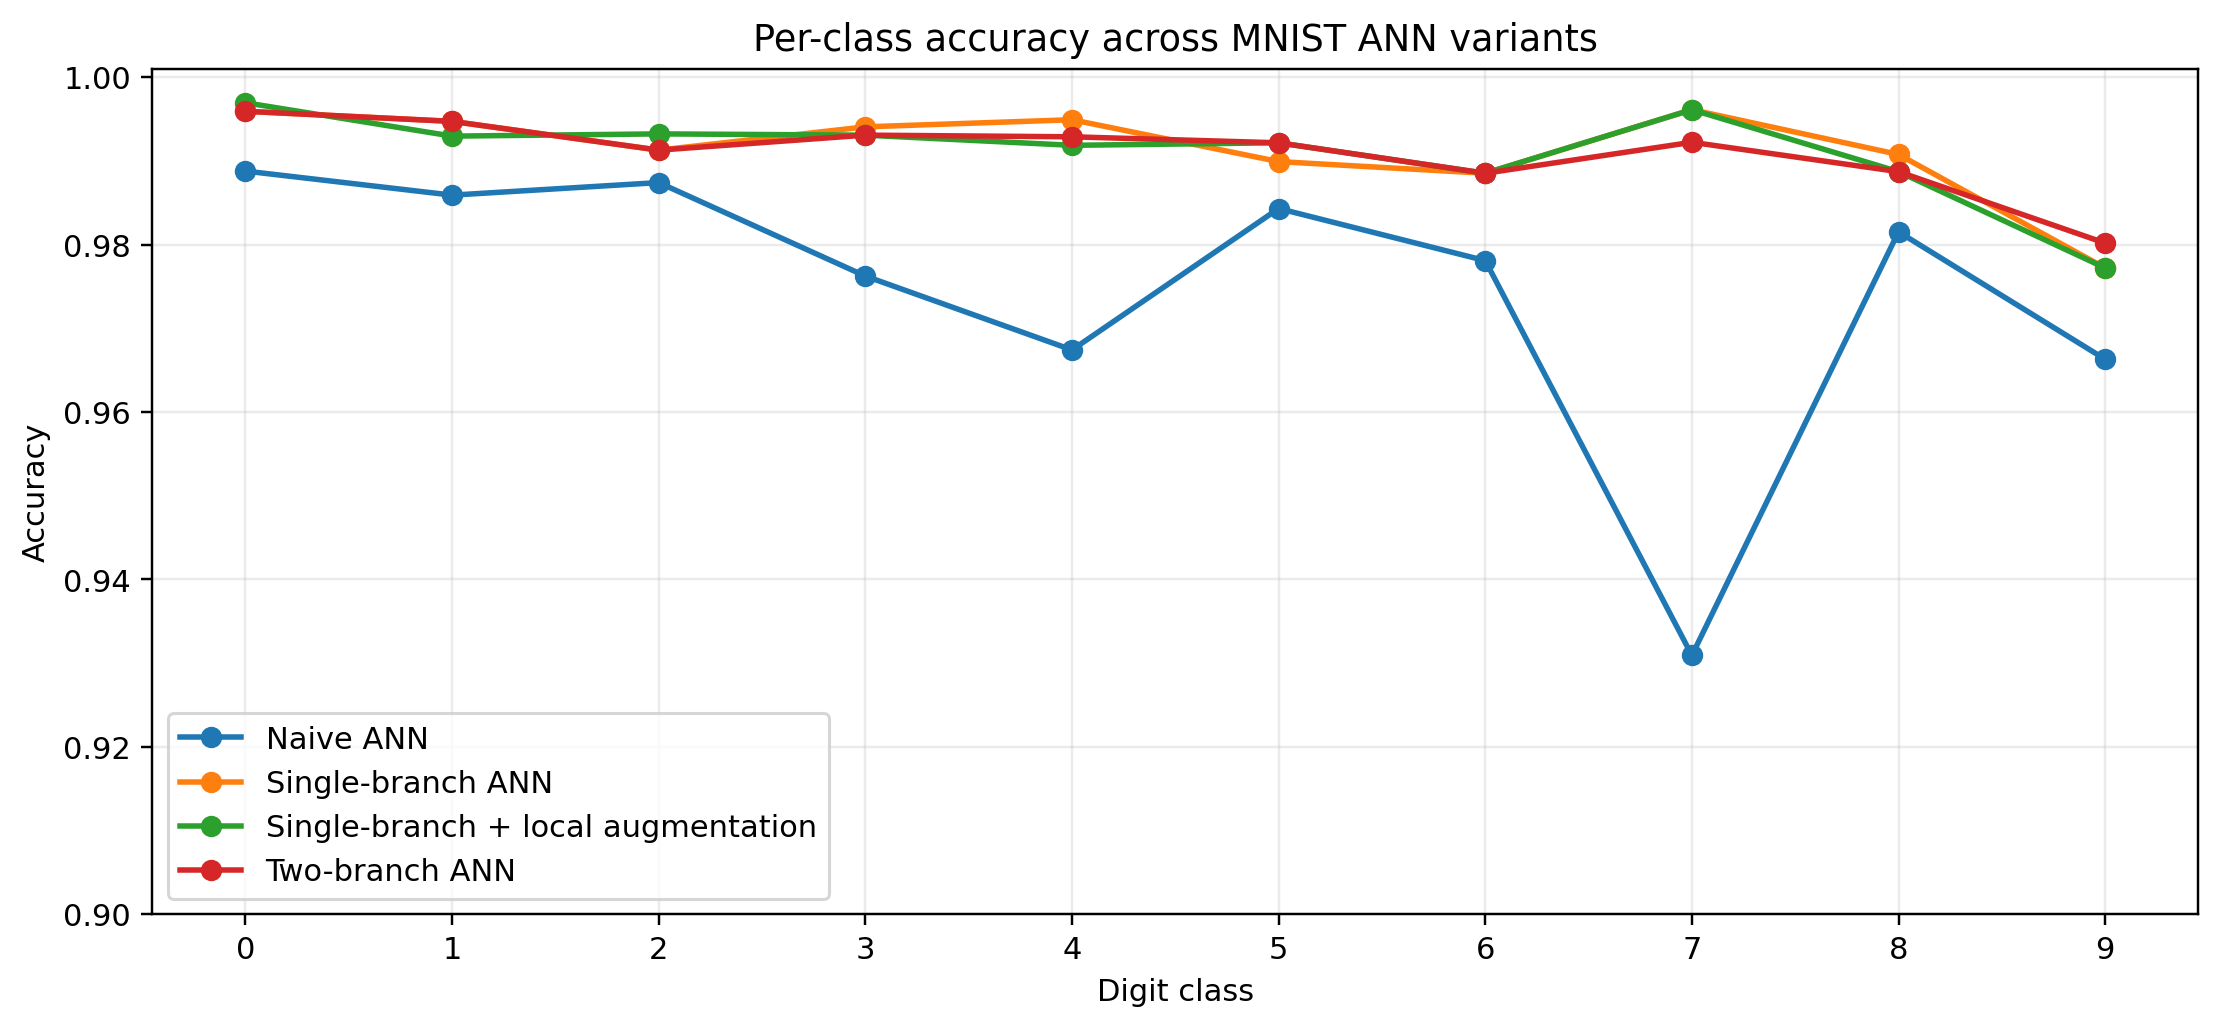
\includegraphics[width=0.92\textwidth]{figures/mnist-models/per_class_accuracy_comparison.png}
  \caption{So sánh accuracy theo từng lớp giữa bốn biến thể ANN trên MNIST.}
  \label{fig:mnist-per-class-comparison}
\end{figure}

Bảng so sánh tổng thể và biểu đồ tổng hợp cho thấy bức tranh rất rõ. Naive ANN là mốc khởi đầu hợp lý nhưng có \textit{generalization gap} lớn nhất và nhạy với biến thiên hình học. Việc thêm \textit{deslant + recenter + HOG + BatchNorm + Dropout} giúp mô hình nhảy vọt từ $97.46\%$ lên $99.14\%$, đồng thời kéo \textit{generalization gap} giảm hơn một nửa. Đây là cải tiến quan trọng nhất, xác nhận rằng phần lớn lợi ích đến từ việc biểu diễn dữ liệu đúng hơn chứ không phải chỉ làm mạng sâu hơn.

Biểu đồ accuracy theo từng lớp cho thấy sau khi thêm tiền xử lý và HOG, độ chính xác tăng gần như đồng đều trên toàn bộ 10 lớp, nhưng các lớp khó nhất vẫn là $9$, $6$ và $8$. Điều này cũng giải thích vì sao augmentation cục bộ chỉ mang lại chênh lệch rất nhỏ: MNIST vốn là bộ dữ liệu tương đối sạch, chữ số khá thẳng và biến thiên hình học toàn cục đã được xử lý phần lớn bởi \textit{deslant + recenter}. Vì vậy, sau khi đã chuẩn hóa hình học và thêm HOG, việc tiếp tục bơm \textit{elastic distortion} hay \textit{stroke jitter} không còn tạo ra thêm nhiều thông tin hữu ích cho mô hình.

Kết luận cho Chương 1 có thể chốt gọn bằng ba ý. Thứ nhất, cấu hình tốt nhất theo test accuracy trong loạt thử nghiệm hiện tại là \textit{Single-branch ANN} với $99.14\%$, nên trên MNIST lợi ích lớn nhất thật sự đến từ \textit{deslant + recenter + HOG} chứ không phải từ việc làm kiến trúc ngày càng phức tạp. Thứ hai, augmentation cục bộ không còn cần thiết sau khi dữ liệu đã được chuẩn hóa hình học; kết quả $99.11\%$ của biến thể có \textit{elastic distortion + stroke jitter} gần như không cải thiện gì so với single-branch gốc. Thứ ba, việc tách raw pixel và HOG thành hai nhánh riêng cũng không mang lại lợi ích thực nghiệm rõ rệt; two-branch ANN chỉ đạt $99.10\%$, thấp hơn nhẹ so với single-branch, cho thấy trong bối cảnh MNIST thì hợp nhất sớm raw pixel và HOG đã là lựa chọn đủ tốt. Vì vậy, insight quan trọng nhất của chương này là: với một bộ dữ liệu sạch như MNIST, ANN thuần vẫn rất hiệu quả nếu được cung cấp đúng biểu diễn đầu vào, còn các cải tiến phức tạp hơn chưa chắc tạo thêm lợi ích đáng kể.
